% Surgical Inference — arXiv build
% Build: tectonic main.tex   (tectonic fetches packages on demand)
% Source of truth for prose: ../Scratchpad/surgical-inference.md
% The conversion agent fills in the sections; keep every number identical to the markdown draft.
\documentclass[11pt]{article}

\usepackage[margin=1in]{geometry}
\usepackage{microtype}
\usepackage{amsmath}
\usepackage{booktabs}
\usepackage{graphicx}
\usepackage{float}
\usepackage{caption}
\usepackage{subcaption}
\usepackage{enumitem}
\usepackage[numbers,sort&compress]{natbib}
\usepackage[colorlinks=true,linkcolor=blue!50!black,citecolor=blue!50!black,urlcolor=blue!50!black,
  pdftitle={Surgical Inference: Decomposing Generative Models for Heterogeneous On-Device SoC Inference},
  pdfauthor={Matt Mireles},
  pdfsubject={On-device generative model inference on Apple Silicon heterogeneous SoCs},
  pdfkeywords={on-device inference, heterogeneous computing, Apple Silicon, Neural Engine, Core ML, model decomposition}
]{hyperref}
\usepackage{xcolor}
\usepackage{tabularx}
\usepackage{seqsplit}

\graphicspath{{figures/}}

% Absorb the occasional unbreakable code token in prose without a visible overrun.
\setlength{\emergencystretch}{3em}

% Inline code styling consistent with the markdown draft's backticks
\newcommand{\code}[1]{\texttt{#1}}
% Breakable variant for long file paths (used inside the appendix listings).
\newcommand{\pth}[1]{\texttt{\seqsplit{#1}}}

% Guarded figure include: build succeeds even when a figure PDF is not yet present.
\newcommand{\pendingfig}[1]{\fbox{\parbox{0.85\linewidth}{\centering\vspace{2em}PENDING FIGURE: \texttt{#1}\vspace{2em}}}}

\title{Surgical Inference: Decomposing Generative Models for\\Heterogeneous On-Device SoC Inference}
\author{Matt Mireles\\Independent Researcher\\\texttt{mattmireles@gmail.com}}
\date{}

\begin{document}
\maketitle

\begin{abstract}
On-device generative inference usually means choosing one backend: CPU for compatibility, GPU for throughput, or an NPU when the compiler accepts the graph. Modern SoCs are heterogeneous computers --- CPU cores, GPU cores, and neural accelerators share memory but differ in execution strengths, admission constraints, and power behavior --- and single-backend deployment leaves most of the chip idle. We present \emph{Surgical Inference}, a deployment methodology that changes the unit of compilation from ``the model'' to a set of fixed-shape neural submodels and native stages: each stage is classified by computational motif, implemented in the simplest suitable form, and assigned to the SoC engine that measurement --- not intuition --- selects.

We evaluate on two structurally opposite generative workloads. Kokoro-82M, a feed-forward text-to-speech pipeline decomposed into four Core ML model families and three native Swift stages, runs \textbf{1.6--2.3$\times$ faster than MLX}, \textbf{2.0--4.0$\times$ faster than PyTorch MPS}, and \textbf{2.5--7.3$\times$ faster than PyTorch CPU} across three Macs, ships unchanged to iPhone --- 30 s of audio in 3.7 s on an iPhone 15 Pro Max, beating the MLX Swift port on every bucket (1.25--1.44$\times$, Release builds, thermally controlled) --- and completes workloads that memory-exhaust the GPU frameworks. Magenta RealTime 2 (\code{mrt2\_small}, 230M parameters), a live-music model with a hard 40 ms/frame streaming deadline, runs faster than real time on the same phone --- a target its upstream GPU-only path does not attempt --- and yields three findings we have not seen documented: the ANE admission cliff for streaming transformers is \emph{in-graph state mutation}, not attention math; tensor layout determines FP16 \emph{numerical survival} per compute unit, not just placement; and per-call cost on weight-bandwidth-bound stages is weight bytes $\div$ DRAM bandwidth on every engine. Instruments traces and paired power profiles verify all-ANE placement with zero app-attributed GPU intervals and a 56\% cut in CPU instructions versus a GPU control.

Negative results are central: a monolithic Core ML export of the first workload does not exist as a valid artifact --- conversion fails at the data-dependent alignment, and the strongest partial monolith is numerically invalid --- the ANE rejected the first workload's largest dense stage on tensor geometry and every stateful variant of the second's transformer, and the decomposed pipelines win anyway. The active ingredients are decomposition, static per-stage compilation, deliberate placement, and validated host glue, not any single accelerator. Code, models, and benchmarks for the first case study are open source, as are the second's conversion exporters, validators, and validation receipts; the full artifact map is given in Appendix~\ref{app:artifacts}.
\end{abstract}

%% Keywords
\noindent\textbf{Keywords:} on-device inference, heterogeneous computing, Apple Silicon, Neural Engine, Core ML, model decomposition, generative models, text-to-speech, music generation, autoregressive streaming, MLX

\section{Introduction}\label{sec:intro}

The deployment of generative models on edge devices has emerged as a critical research direction, motivated by privacy, latency, network independence, energy cost, and user experience. The hardware is already heterogeneous. Apple Silicon integrates CPU cores, GPU cores, and a dedicated neural network accelerator (the Apple Neural Engine, or ANE) on a single die with unified memory. Similar CPU/GPU/NPU structures now exist across phones, laptops, tablets, and embedded systems.

Despite this hardware heterogeneity, the dominant approach to local AI inference on Apple Silicon uses Metal-based engines (Ollama/llama.cpp, MLX, PyTorch MPS) that target the GPU. That default is rational: the GPU is programmable, high-throughput, and forgiving. But it also creates a systems bottleneck. A GPU-only model competes with the user interface, rendering, media pipelines, and any concurrent local LLM. The neural accelerator remains mostly idle, CPU vector units are underused, and the application has fewer ways to trade latency, energy, and thermals.

The common alternative --- compile the whole model to a neural accelerator --- is too simple. Neural accelerators are fast and power-efficient for the graphs they admit, but their compilers impose static-shape, op-set, and tensor-geometry constraints. A modern generative model is rarely one homogeneous graph. It often contains dense feed-forward blocks, small recurrent or autoregressive components, data-dependent indexing, masking, DSP, sampling, and post-processing. Some of these parts are excellent neural-accelerator candidates. Some are better as native CPU code. Some should stay on GPU. Treating the model as a single scheduling unit hides this structure.

We argue that the deployment unit should be the \emph{inference pipeline}, not the original model file. Surgical Inference decomposes a generative pipeline into smaller compiled submodels and native stages, then schedules them deliberately across the SoC. The procedure assumes only a heterogeneous SoC whose accelerators impose admission constraints, and applies when a model contains separable stages whose dataflow can be made explicit; the constraint catalog we document is Apple-specific, and all measurements in this paper are on Apple Silicon (\S\ref{sec:disc-limitations}). We measure it on two case studies chosen to stress different regimes. Text-to-speech (Kokoro-82M) is a clean batch example: recurrent prosody prediction, duration-dependent expansion, pitch/noise prediction, harmonic DSP, and dense convolutional waveform generation all coexist in one reference model. Live music generation (Magenta RealTime 2) adds the constraint the first lacks: a hard 40 ms autoregressive deadline that never pauses, on a phone, where a missed frame is an audible dropout rather than a slower benchmark row.

The systems objective is broader than raw latency. A decomposed pipeline can reduce wall-clock time, avoid GPU-only memory blowups, overlap CPU work with neural inference, and lower GPU residency so other workloads --- including a local LLM --- can run concurrently. This paper measures latency and completion behavior directly for both case studies, and --- for the second --- power and placement directly: paired Power Profiler captures and Instruments residency traces on physical iPhones (\S\ref{sec:cs2-power}), including a thermal-soak result that currently fails and is reported as such. Shorter end-to-end execution, bounded memory use, and partial use of CPU/ANE instead of continuous GPU occupancy are the deployment properties that make lower-energy, cooler on-device inference plausible; the second case study turns part of that plausibility argument into measurement.

We introduce \emph{Surgical Inference} and make four contributions:

\begin{enumerate}[leftmargin=*]
\item \textbf{A decomposition methodology} for multi-stage generative pipelines on heterogeneous SoCs: a three-motif classification --- Sequential-Dynamic, Data-Dependent Logic, Dense-Static --- a decomposition procedure, and a per-stage placement ablation whose results overrode intuition in both case studies, in opposite directions (\S\ref{sec:method}, \S\ref{sec:disc-ane}).

\item \textbf{Two complete implementations with cross-device empirical validation.} A Kokoro-82M pipeline --- four Core ML model families, three native Swift stages, zero Python at inference time --- benchmarked on three Macs (M1 Mini, M2 Air, M2 Ultra) and two iPhones (A14, A17 Pro) against MLX, PyTorch MPS, PyTorch CPU, and two independent Core ML Kokoro ports (\S\ref{sec:cs1}--\ref{sec:cs1-eval}); and a Magenta RealTime 2 streaming pipeline holding a 25 Hz autoregressive deadline on a phone (\S\ref{sec:cs2}). Negative results are reported as results: a valid monolithic Core ML export of Kokoro-82M does not exist --- conversion fails at the data-dependent alignment and the strongest partial monolith is numerically invalid (\S\ref{sec:cs1-monolith}); the vocoder's categorical ANE rejection on tensor geometry (\code{ANECCompile() FAILED} on every device tested); \code{.all}'s silent fallback on macOS and hard failure on iOS; the GPU frameworks' OOM/jetsam failures on constrained memory; and the finding that naive native DSP ports regress until engineered (a 12$\times$ hn-nsf speedup from eliminating protocol-dispatched RNG, \S\ref{sec:dsp}).

\item \textbf{Three undocumented ANE admission findings} from the streaming case study: in-graph \emph{state mutation} --- not attention math --- is the compile-time cliff for streaming transformers, located by a falsification ladder and escaped by restructuring the transformer as a stateless step function (\S\ref{sec:cs2-state}); tensor layout governs FP16 \emph{numerical survival} per compute unit --- after a channels-first rewrite the ANE was the only engine producing finite codec output (\S\ref{sec:cs2-layout}); and on weight-bandwidth-bound stages per-call cost is weight bytes $\div$ DRAM bandwidth on every compute unit, an invariant that reshaped the sampling loop from twelve predictions per frame into one (\S\ref{sec:cs2-bandwidth}).

\item \textbf{Direct residency and energy instrumentation}, addressing what model-level scheduling claims usually leave unproven: Instruments Core ML traces showing per-model ANE hardware intervals and \emph{zero} app-attributed Metal GPU intervals, turned into a machine-checkable placement-evidence artifact, plus paired Power Profiler captures showing the all-ANE policy removes process GPU impact and roughly halves CPU instructions versus a temporal-GPU control (\S\ref{sec:cs2-power}).
\end{enumerate}

All code, pre-converted Core ML models, and benchmark data for the first case study are available at:
\begin{itemize}[leftmargin=*]
\item \url{https://github.com/mattmireles/kokoro-coreml}
\item \url{https://huggingface.co/mattmireles/kokoro-coreml}
\end{itemize}

The second case study's conversion and validation layer is public at \url{https://github.com/mattmireles/magenta-realtime-2-iphone} --- including the corrected exporters that reproduce the \S\ref{sec:cs2-state}--\S\ref{sec:cs2-bandwidth} findings, the superseded exporters retained as negative-result artifacts, numerical-parity validators, reference fixtures, and validation receipts, with pre-converted packages mirrored on \href{https://huggingface.co/mattmireles/magenta-realtime-2-iphone}{Hugging Face} (generation status per artifact in Appendix~\ref{app:artifacts}). The streaming runtime and instrumentation live in the Crossfade repository, a fork of \href{https://github.com/magenta/magenta-realtime}{magenta/magenta-realtime} that is private at the time of writing; the full artifact and reproduction map is given in Appendix~\ref{app:artifacts}.

\section{Background}\label{sec:background}

\subsection{Heterogeneous SoCs as Inference Targets}\label{sec:soc}

Apple's M-series and A-series SoCs integrate three relevant compute units on a single die with unified memory architecture (UMA). All three compute units access the same physical memory pool, which removes explicit device-to-device copy costs but does not make the compute units interchangeable. Each engine has a different instruction model, scheduling overhead, admission policy, and power profile.

\textbf{CPU.} Performance and efficiency cores optimized for sequential and branching workloads. Excellent at data-dependent control flow, dynamic shapes, and small-batch operations. The Accelerate framework provides vectorized DSP routines (vDSP) and BLAS operations.

\textbf{GPU.} Tile-based deferred renderer with compute shader support via Metal. Optimized for parallelizable workloads with flexible kernel programming through Metal Performance Shaders (MPS) and the MLX framework. Handles dynamic shapes and arbitrary computation graphs.

\textbf{Neural Engine (ANE).} Fixed-function matrix accelerator designed for high-throughput, low-power neural network inference. Accelerates a constrained subset of operations --- convolutions, matrix multiplications, elementwise ops, pooling, normalization --- under strict requirements:

\begin{itemize}[leftmargin=*]
\item \textbf{Static shapes.} All tensor dimensions must be known at compile time.
\item \textbf{Supported op set.} Operations outside the ANE-accepted set trigger fallback to CPU/GPU.
\item \textbf{No data-dependent control flow.} Loops and conditionals depending on tensor values cannot execute on ANE.
\item \textbf{Tensor geometry limits.} Per-axis dimensions are bounded (community documentation and our own compiler errors place the limit at 16,384 elements per axis); large intermediate activations that exceed ANE SRAM incur DRAM round-trips.
\end{itemize}

These constraints make the ANE ideal for dense, regular, feed-forward computation at moderate tensor sizes --- but, as we show in \S\ref{sec:disc-ane}, ``dense and static'' is necessary, not sufficient. Audio-rate tensors (hundreds of thousands of samples on the last axis) can categorically exceed ANE admission limits, in-graph state mutation can fail compilation outright (\S\ref{sec:cs2-state}), and FP16 numerical health can depend on internal layout (\S\ref{sec:cs2-layout}). The practical inference target is therefore not ``the ANE'' or ``the GPU''; it is the whole SoC, with stages mapped to engines according to what the compiler accepts and what measurement validates.

\subsection{GPU-Centric Deployment and Its Blind Spot}\label{sec:gpu-centric}

The prevailing practice for local ML inference on Apple Silicon has converged on GPU-centric execution through Metal-based frameworks:

\begin{itemize}[leftmargin=*]
\item \textbf{llama.cpp / GGML}~\citep{llamacpp}. The engine underlying Ollama and many local LLM tools. Uses Metal shaders directly. CPU and GPU only.
\item \textbf{MLX}~\citep{mlx}. Apple's own NumPy-like framework for Apple Silicon. Purpose-built for the architecture but GPU-only; it cannot dispatch to the ANE.
\item \textbf{PyTorch MPS}~\citep{pytorch-mps-metal,pytorch-mps-notes}. Apple's Metal Performance Shaders backend for PyTorch. GPU only. Transparent fallback to CPU for unsupported operations.
\item \textbf{Core ML}~\citep{coremltools}. Apple's conversion and runtime framework. Capable of dispatching to CPU, GPU, or ANE. Used extensively for small on-device models but rarely for generative workloads. Its scheduler partitions graphs across compute units opaquely, and rejected ANE subgraphs fall back \emph{silently} --- a model ``running on the ANE'' may not be.
\end{itemize}

The conventional wisdom --- reinforced by LLM-dominated discussion in the on-device ML community --- holds that Core ML provides no meaningful benefit for generative inference. This is often true for large autoregressive language models: they are memory-bandwidth-bound, and the ANE does not create additional memory bandwidth beyond unified memory. But that conclusion does not transfer to all generative systems. Many models are not one uniform transformer loop. They are pipelines with separable dense, sequential, and data-dependent regions. GPU-only deployment collapses these regions back into a single queue on the GPU, monopolizing the most generally useful accelerator even when other SoC engines could do part of the work.

\subsection{Kokoro-82M: The First Case Study}\label{sec:kokoro-bg}

Kokoro-82M~\citep{kokoro-model,kokoro-lib} is a lightweight text-to-speech model released by hexgrad under Apache 2.0, based on the StyleTTS 2 architecture~\citep{styletts2}. Despite only 82 million parameters, it achieves quality competitive with much larger models in community evaluations by leveraging efficient StyleTTS 2 components and an iSTFTNet-based decoder~\citep{istftnet}.

We use Kokoro-82M as a case study because it is small enough to ship on phones, high quality enough to matter, and structurally heterogeneous. The reference inference path contains seven conceptual stages:

\begin{enumerate}[leftmargin=*]
\item \textbf{Duration prediction.} A BERT-based text encoder feeds a prosody predictor (LSTM + CNN stack) that produces per-phoneme durations, text encodings, and style features.
\item \textbf{Duration-dependent expansion.} Predicted durations expand token-level features into acoustic frames.
\item \textbf{Prosody (F0/N) prediction.} A small convolutional network predicts pitch (F0) and noise (N) contours from aligned features and style embedding.
\item \textbf{Decoder pre-processing.} The decoder's encode and decode blocks (convolutional residual stacks with style-conditioned AdaIN normalization) produce pre-vocoder features.
\item \textbf{Harmonic source generation (hn-nsf).} A SineGen-based module converts the F0 contour into a harmonic waveform, then applies STFT to produce spectral features used by the vocoder.
\item \textbf{Vocoder (GeneratorFromHar).} The final convolutional stack combines pre-vocoder features with harmonic features and produces the output waveform via iSTFT.
\item \textbf{Trim.} Output is trimmed to the target audio length.
\end{enumerate}

The original PyTorch reference implementation executes all seven stages on CPU or GPU/MPS through one eager runtime, with significant Python overhead between stages. Surgical Inference asks a different question: which of these stages should remain a model, which should become native code, and which SoC engine should each stage use?

\subsection{Magenta RealTime 2: The Second Case Study}\label{sec:mrt2-bg}

Magenta RealTime 2 (MRT2)~\citep{magenta-rt,magenta-rt-repo} is Google's open-weights live-music model. Unlike a TTS model that renders a finished utterance, MRT2 \emph{streams}: a decoder-only transformer autoregressively generates one frame of 12 residual-vector-quantization (RVQ) tokens every 40 ms, and a SpectroStream codec decoder --- in the RVQ lineage of SoundStream~\citep{soundstream} --- converts each token frame into 1,920 samples of 48 kHz stereo PCM. Generation is steerable in real time by text, audio, and MIDI conditioning. The upstream project ships real-time inference through MLX --- GPU-only --- and supports it exclusively on M-series Macs; there is no phone target.

We use the smallest configuration, \code{mrt2\_small} (230M parameters), as the second case study because it is the structural complement of the first. Kokoro is feed-forward and batch: the deployment metric is wall time for a finished artifact, and every stage runs once per utterance. MRT2 is autoregressive and streaming: frame \emph{N+1} cannot start before frame \emph{N}'s tokens exist, the audio clock never pauses, and the deployment metric is sustained p99 frame time against a 40 ms deadline. It also exercises the one motif the first case study could route around: a stateful transformer with per-frame K/V-cache updates on the hot path (41-frame local-attention windows across 12 temporal layers, plus a 12-level serial depth sampler per frame). If the methodology only works when the Sequential-Dynamic motif can be left on the CPU, this workload exposes that.

\section{Surgical Inference Methodology}\label{sec:method}

Surgical Inference is a deployment-time graph partitioning method. It does not change model weights or retrain the network. It changes the compiled artifact boundary. A single reference model becomes a small number of fixed-shape neural packages plus native kernels for dynamic or irregular work. The method is intentionally simple:

\begin{itemize}[leftmargin=*]
\item Cut only at real dataflow boundaries.
\item Preserve numerical equivalence at each cut.
\item Let measured stage placement override intuition.
\item Optimize the host glue because it becomes part of the model.
\item Use concurrency only where the data dependencies prove it is safe.
\end{itemize}

\subsection{Computational Motifs}\label{sec:motifs}

We classify stages into three motifs, each with a characteristic hardware affinity:

\textbf{Motif 1: Sequential-Dynamic (SD).}
Characterized by recurrent layers (LSTMs, GRUs), autoregressive decoding with KV-cache, sampling loops, beam search, or computations where step \emph{t} depends on step \emph{t$-$1}. Tensor shapes may vary across inputs. Examples: LSTM-based duration prediction in Kokoro, autoregressive transformer decoding in LLMs, diffusion samplers with step-wise scheduler state.

\emph{Hardware affinity:} \textbf{CPU or GPU} --- as inherited. But the motif is a property of the boundary you draw, not the stage you inherit: when the sequential dependency is only cache state, the per-step math is Dense-Static and the recurrence is Data-Dependent Logic that can move to the host. Case study 2 shows this decomposition-within-a-stage unlocking ANE compilation for a streaming transformer (\S\ref{sec:cs2-state}).

\textbf{Motif 2: Data-Dependent Logic (DDL).}
Computations whose \emph{structure} depends on tensor values, not just their shapes. Examples: duration-dependent expansion, top-k filtering, token suppression, dynamic masking, bucketing, ragged sequence packing, audio trimming, or branchy post-processing.

\emph{Hardware affinity:} \textbf{CPU (native Swift/C).} Too small and too irregular for GPU or ANE dispatch to amortize. Best implemented directly, not through a tensor runtime.

\textbf{Motif 3: Dense-Static (DS).}
Large blocks of convolutions, matrix multiplications, attention with fixed shapes, normalization, upsampling, or elementwise ops with shapes fully known at compile time and no data-dependent branching. Examples: convolutional vocoders, image decoders, denoisers, fixed-shape encoders, codec decoders, and BERT-style encoders with fixed input sizes.

\emph{Hardware affinity:} \textbf{Core ML, with placement determined empirically.} Dense-Static work is the candidate set for ANE acceleration, but the ANE's admission constraints (op set, tensor geometry limits, SRAM budget) are checked at compile time per stage. A Dense-Static stage that the ANE rejects still benefits from Core ML compilation --- fused fp16 kernels and ahead-of-time graph optimization on CPU+GPU --- relative to eager-mode GPU frameworks. Placement is a measurement, not an assumption.

\subsection{Decomposition Procedure}\label{sec:procedure}

Given a generative pipeline, apply the following procedure:

\begin{enumerate}[leftmargin=*,label=\arabic*.]
\item Trace or instrument the reference forward pass and identify real dataflow boundaries:
  \begin{itemize}[leftmargin=1.5em]
  \item values whose shape or semantics are stable enough to validate
  \item boundaries where data-dependent logic enters or leaves the graph
  \item independent branches that can run concurrently
  \end{itemize}

\item For each stage, classify its computational motif (SD, DDL, DS).

\item For stages classified as Dense-Static:
  \begin{itemize}[leftmargin=1.5em]
  \item Enforce static shapes via bucketing if necessary
  \item Export as a Core ML \code{.mlpackage}
  \item Validate numerical equivalence (correlation $>$ 0.99 vs PyTorch)
  \item Ablate compute-unit placement per stage: try \code{.cpuAndNeuralEngine}, \code{.cpuAndGPU}, and \code{.all}; keep the fastest placement that passes the task validation gate. Do not trust \code{.all} to mean ``ANE'': rejected subgraphs fall back silently.
  \end{itemize}

\item For stages classified as Data-Dependent Logic:
  \begin{itemize}[leftmargin=1.5em]
  \item Implement natively in Swift (or C)
  \item Use Accelerate/vDSP for vectorizable DSP
  \item Profile the native implementation: a naive port is often slower than PyTorch until optimized
  \end{itemize}

\item For stages classified as Sequential-Dynamic:
  \begin{itemize}[leftmargin=1.5em]
  \item If the recurrence is only cache state, restructure as a stateless step function: caches as ordinary inputs, current-step updates as ordinary outputs, host owns mutation and continuity. The remaining graph is Dense-Static; classify it as such (\S\ref{sec:cs2-state})
  \item If small, export as Core ML and measure CPU/GPU/ANE-adjacent policies anyway; the compiler may fuse useful subgraphs
  \item If large and memory-bandwidth-bound, expect per-call cost $\approx$ weight bytes $\div$ DRAM bandwidth on EVERY compute unit; minimize weight re-streaming (fewer calls, lower precision) before chasing placement (\S\ref{sec:cs2-bandwidth})
  \item If latency is dominated by host dispatch, prefer fewer calls
  \end{itemize}

\item Orchestrate the pipeline in Swift, with explicit model loading, tensor handoff via \code{MLMultiArray}, and inline timing of each stage. Profile the host-side glue: tensor materialization and padding are real costs. Where the dataflow allows, run CPU stages concurrently with Core ML predicts --- heterogeneous units can genuinely overlap, and the decomposition makes the independence explicit.

\item Benchmark the assembled pipeline against:
  \begin{itemize}[leftmargin=1.5em]
  \item The original PyTorch baseline (CPU and GPU/MPS)
  \item GPU-native frameworks (MLX)
  \item Any existing Core ML implementations of the same model
  \item A monolithic conversion of the full model, if one can be built at all --- the attempt itself is evidence (\S\ref{sec:cs1-monolith})
  \item Across a range of input lengths and target hardware
  \item With power/thermal instrumentation when energy claims are made
  \end{itemize}
\end{enumerate}

Step 3's ablation clause is load-bearing. In the first case study it changed the shipped configuration: the empirically fastest valid policy places only one of the four Core ML model families on the ANE (\S\ref{sec:disc-ane}). In the second case study the same clause ran the other way --- measurement moved stages \emph{onto} the ANE that the motif taxonomy had written off (\S\ref{sec:cs2-state}) and revealed that for one stage the ANE was the only numerically correct placement (\S\ref{sec:cs2-layout}). A paper that merely says ``we used the Neural Engine'' would be wrong in both directions; the correct statement is that each pipeline uses the whole SoC deliberately.

\subsection{CPU-Side DSP: A Non-Obvious Optimization Challenge}\label{sec:dsp}

A subtle consequence of the decomposition procedure: when a stage is classified as DDL or must remain on CPU due to Core ML incompatibility, the naive Swift implementation is often \emph{slower} than the PyTorch CPU reference. PyTorch's underlying numerical libraries are highly optimized; a direct Swift port without equivalent optimization will regress.

We observed this acutely with the hn-nsf harmonic source module. The initial Swift port ran at 166 ms for 3 s of audio --- nearly 4$\times$ slower than PyTorch. Profiling identified per-sample Gaussian RNG, dispatched through Swift's \code{RandomNumberGenerator} protocol, as the dominant cost (154 ms across 648k calls). Replacing this with a bulk pre-allocated noise buffer using direct xorshift64 reduced hn-nsf to 14 ms --- a 12$\times$ speedup with identical numerical output. Subsequent vDSP vectorization of the noise/mask path and a frame-rate source-phase reformulation reduced it further; in the current pipeline hn-nsf costs roughly 9 ms at the 3 s bucket on M2 Ultra.

This observation generalizes: \textbf{any Swift DSP port must be profiled and optimized with the same rigor as neural network inference.} Use Accelerate/vDSP for vectorizable operations. Use double precision for quantities that accumulate (phase, in cumulative sine generation). Pre-allocate buffers. Eliminate protocol dispatch in hot loops. The methodology explicitly incorporates this optimization pass; skipping it produces pipelines that are worse than the PyTorch baseline they are meant to replace.

\subsection{Host-Side Materialization Cost}\label{sec:host-cost}

Decomposing a pipeline across multiple Core ML models and Swift stages introduces host-side overhead: model dispatch, tensor format conversion, padding to bucket geometry, and Swift-level control flow between stages. This cost is not negligible and it is easy to get wrong. Two host-side bugs in early versions of the Kokoro pipeline each cost more than any model stage: a one-hot alignment expansion implemented as a dense matrix multiply through zeros (later made sparse, and ultimately eliminated --- the shipped code expands token vectors directly into frame buffers with no matrix at all), and boxed \code{MLMultiArray} element reads over a strided \code{Float16} waveform during trim. Both were invisible to model-level profiling and were found only by timing the full synthesize call. The methodology therefore times the \emph{end-to-end} wall clock as the primary metric, with per-stage timings as diagnostics.

The second case study escalates this from a performance concern to a correctness concern: host glue that misreads strided Core ML outputs, or feeds a stateful graph inputs it silently ignores, can pass every model-level validation and still destroy output quality (\S\ref{sec:cs2-host}). The procedure's validation step therefore extends past the graph boundary --- every host-side consumer of a model output must be validated against the reference at least once, and stateful graphs need cross-prediction tests proving the state is actually read.

\section{Case Study 1: Kokoro-82M Pipeline}\label{sec:cs1}

\subsection{Applying the Procedure}\label{sec:cs1-procedure}

We apply the decomposition procedure from \S\ref{sec:procedure} to Kokoro-82M. The resulting pipeline is shown in Figure~\ref{fig:kokoro-pipeline}.

\begin{figure}[H]
\centering
\IfFileExists{figures/fig-kokoro-pipeline.pdf}{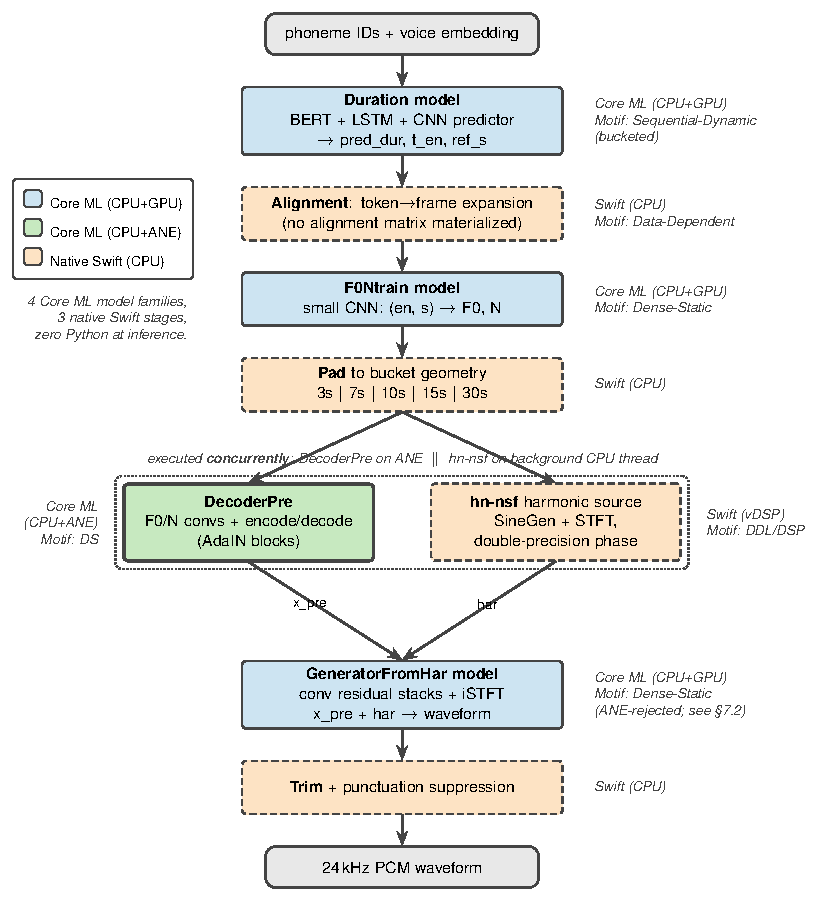
\includegraphics[width=0.8\linewidth]{fig-kokoro-pipeline}}{\pendingfig{fig-kokoro-pipeline}}
\caption{The decomposed Kokoro-82M pipeline: four Core ML model families and three native Swift stages, zero Python at inference time. Each stage is classified by computational motif and placed on the SoC engine that measurement selects (color = placement); only DecoderPre is admitted to the ANE, while the geometry-rejected GeneratorFromHar and the sequential Duration model run Core ML on CPU+GPU. The decomposition also exposes cross-unit parallelism a monolithic graph cannot express: DecoderPre (ANE) and the hn-nsf harmonic source (background CPU thread) execute concurrently.}
\label{fig:kokoro-pipeline}
\end{figure}

\textbf{Four Core ML model families, three Swift stages, zero Python at inference time.} The per-stage compute-unit annotations above are the shipped \emph{staged} policy, hard-coded in the pipeline's model loading, and the outcome of the \S\ref{sec:procedure} ablation: DecoderPre loads with \code{.cpuAndNeuralEngine}; Duration, F0Ntrain, and GeneratorFromHar load with \code{.cpuAndGPU}. Section~\ref{sec:disc-ane} explains why this --- and not an all-ANE plan --- is the empirically correct configuration.

Two structural points the diagram encodes. First, the alignment ``matrix'' no longer exists in the hot path: predicted durations drive a direct token-vector-to-frame expansion, so neither the one-hot matrix nor the matrix multiplies (\code{en = d @ align}, \code{asr = t\_en @ align}) are ever materialized (the matrix construction survives only as a debug-dump path). Second, DecoderPre and hn-nsf execute \emph{concurrently}: the harmonic source depends only on the padded F0 contour, so it runs on a background CPU thread while the DecoderPre Core ML predict is in flight, and the pipeline accounts for the overlap explicitly in its stage timings. The decomposition does not just place stages on the right compute unit --- it exposes cross-unit parallelism a monolithic graph cannot express.

For texts longer than one bucket, a caller-side chunking layer splits input at a fixed token cap and joins the per-chunk PCM; the benchmarks in \S\ref{sec:cs1-eval} time single synthesize calls.

\subsection{Core ML Export Details}\label{sec:cs1-export}

All Core ML models were exported via \code{coremltools} 8.3.0~\citep{coremltools,coremltools-pytorch} (PyTorch pinned at 2.5.0 for export) with \code{compute\_precision=FLOAT16}. Key export decisions:

\begin{itemize}[leftmargin=*]
\item \textbf{Duration model} is exported at enumerated token sizes (32, 64, 128, 256, 320, 384, 512) to accommodate inputs up to 30 seconds; the E5RT runtime does not handle RangeDim/EnumeratedShapes efficiently, forcing per-size packages. The runtime additionally supports \emph{exact-duration} packages (e.g. \code{kokoro\_duration\_exact\_t156}) generated for known token lengths, which avoid padded-graph compute; these are an environment-gated opt-in used by the benchmark adapters, while the library's production default remains the padded mask-aware packages. Padded duration graphs are expensive: in an early benchmark configuration, the padded duration stage alone cost 82--733 ms per call on M2 Ultra before the exact-duration path eliminated it.

\item \textbf{F0Ntrain, DecoderPre, and GeneratorFromHar} are exported at five bucket sizes targeting 3 s, 7 s, 10 s, 15 s, and 30 s of audio (F0Ntrain at frame counts t120/t280/t400/t600/t1200). The bucket is selected at runtime as the smallest that fits the predicted duration.

\item \textbf{AdaIN compatibility.} Early decoder-only exports failed due to MIL broadcast issues with AdaIN layers, forcing IdentityAdaIN workarounds that degraded quality. Re-export with the decomposed DecoderPre model succeeded with full AdaIN and correlation 1.000000 vs PyTorch --- suggesting the earlier failure was graph-size dependent rather than an AdaIN-specific issue.

\item \textbf{Numerical validation.} All Core ML models were validated against the PyTorch reference with correlation $>$ 0.9999 on test inputs. The benchmark harness additionally enforces a waveform health gate, and published configurations passed human listening checks. A structured blind perceptual evaluation of the end-to-end pipeline (\S\ref{sec:disc-limitations}) later surfaced two real quality deviations that per-stage matched-input correlation cannot see; stage-boundary tensor bisection traced them to three implementation defects --- a native post-process silencing speech-bearing spans, a one-sided inverse-STFT scaling error in the export-time STFT substitution, and a compounding RNG absorbing-state bug in the harmonic-source noise generator. All three were fixed; all four frozen inputs now pass the blind evaluation.
\end{itemize}

\subsection{Swift Stages}\label{sec:cs1-swift}

\begin{itemize}[leftmargin=*]
\item \textbf{Alignment} replaces PyTorch's \code{repeat\_interleave} $\rightarrow$ one-hot $\rightarrow$ matmul chain with direct expansion: each token's hidden vector is copied into its \code{pred\_dur[i]} frame slots, in both token-major (\code{d} $\rightarrow$ \code{en}) and channel-major (\code{t\_en} $\rightarrow$ \code{asr}) layouts, with raw-pointer fast paths for contiguous \code{float32} arrays. This evolved in two steps --- a dense matmul (the \S\ref{sec:host-cost} bug), then a sparse formulation, then no matrix at all.

\item \textbf{hn-nsf} implements SineGen (harmonic sine wave generation from F0) and STFT natively using Accelerate/vDSP. Key implementation details, each visible in the shipped source:
  \begin{itemize}[leftmargin=1.5em]
  \item Double precision (\code{Double}) for phase accumulation; single precision (\code{Float}) for output. Phase drift compounds over hundreds of thousands of samples; double precision is load-bearing.
  \item A \emph{frame-source phase} fast path: the original port upsampled F0 by 300$\times$ and immediately downsampled the phase increments back --- for the model's exact nearest-neighbor geometry these cancel, so the current code computes phase increments directly per F0 frame (waveform-preserving, with the legacy RNG draw order kept for bit-compatible noise).
  \item Bulk noise generation into a pre-allocated buffer using xorshift64 directly, rather than Swift's \code{RandomNumberGenerator} protocol; the Gaussian noise and voiced/unvoiced mask paths are vDSP-vectorized.
  \item The 20-point Hann-window STFT uses a precomputed windowed DFT basis (built once, cached) and vectorized decimated dot products, matching PyTorch's \code{center=True} replicate padding.
  \item Runs concurrently with DecoderPre (\S\ref{sec:cs1-procedure}), so its remaining cost is partly hidden behind the Core ML predict.
  \item Correlation $>$ 0.99 vs PyTorch reference on all test inputs.
  \end{itemize}

\item \textbf{Trim} slices the output waveform to the natural utterance length computed from the duration frames, reading the strided \code{Float16} output buffer directly rather than through boxed \code{MLMultiArray} accessors (the second host-side bug from \S\ref{sec:host-cost}). It then applies a small audio-quality post-process: punctuation tokens own real predicted duration (that is how pauses survive synthesis), and the split Core ML decoder can emit short transients in those spans, so the pipeline fades punctuation-owned spans to silence with $\approx$5 ms ramps while preserving the predicted timing.
\end{itemize}

The pipeline also pools and reuses input \code{MLMultiArray} buffers across calls (zeroed, then filled via \code{memcpy} over contiguous strides) rather than allocating fresh feature arrays per synthesis --- part of the host-materialization discipline from \S\ref{sec:host-cost}.

\section{Case Study 1 Evaluation}\label{sec:cs1-eval}

\subsection{Experimental Setup}\label{sec:cs1-setup}

\textbf{Hardware.} Three Apple Silicon Macs spanning the consumer-to-workstation range (Table~\ref{tab:cs1-hw}), plus two iPhones (\S\ref{sec:cs1-iphone}):

\begin{table}[h]
\centering
\caption{Case Study 1 evaluation hardware: three Apple Silicon Macs spanning the consumer-to-workstation range.}
\label{tab:cs1-hw}
\begin{tabular}{llllrr}
\toprule
Machine & CPU & GPU & ANE & Memory & Bandwidth \\
\midrule
M1 Mac Mini & 8-core (4P+4E) & 8-core & 16-core & 16 GB & 68 GB/s \\
M2 MacBook Air & 8-core (4P+4E) & 10-core & 16-core & 24 GB & 100 GB/s \\
M2 Ultra Mac Studio & 24-core (16P+8E) & 76-core & 32-core & 64 GB & 800 GB/s \\
\bottomrule
\end{tabular}
\end{table}

\textbf{Software.} Swift 6.x; PyTorch 2.5--2.6; coremltools 8.x. The June 2026 external bakeoff (\S\ref{sec:cs1-headline}, \S\ref{sec:cs1-mlx}, \S\ref{sec:cs1-coreml-ports}) ran on macOS 26.5 (Studio) and 15.7.7 (Air, Mini); the April 2026 PyTorch ledger (\S\ref{sec:cs1-pytorch}) ran on the then-current stable releases. All benchmarks run with the machine plugged in and other applications closed.

\textbf{Inputs.} Five frozen text inputs targeting the five runtime buckets, all using the same voice preset (\code{af\_heart}), speed = 1.0:

\begin{table}[h]
\centering
\caption{Frozen text inputs and their target runtime buckets for Case Study 1.}
\label{tab:cs1-inputs}
\begin{tabular}{lrl}
\toprule
Key & Audio duration & Bucket \\
\midrule
3s  & 2.80 s  & 3s \\
7s  & 6.75 s  & 7s \\
10s & 9.60 s  & 10s \\
15s & 13.90 s & 15s \\
30s & 27.38 s & 30s \\
\bottomrule
\end{tabular}
\end{table}

\textbf{Timing boundary.} From immediately before the synthesis call until full PCM audio is materialized in memory --- token IDs in, 24 kHz waveform out (Table~\ref{tab:cs1-inputs} gives the five frozen inputs targeting these buckets; Appendix~\ref{app:boundaries} gives the exact boundary shared across all comparison implementations). Process startup, model download, and playback are excluded. All reported numbers are \emph{warm} medians: models preloaded and primed, first-use Core ML compile/cache effects discarded.

\textbf{Configurations.}

\begin{itemize}[leftmargin=*]
\item \textbf{F. Surgical (this work).} The full Swift + Core ML pipeline, staged compute policy, exact-duration model discovery enabled (the benchmark adapter's default; the library's production default uses the padded duration packages, \S\ref{sec:cs1-export}).
\item \textbf{MLX.} Blaizzy/mlx-audio~\citep{mlx-audio} 0.4.3 at commit \code{862dfbe}, running \code{mlx-community/Kokoro-82M-bf16}. The default MLX deployment path for Kokoro.
\item \textbf{A. Python HAR-post hybrid.} The prior production pipeline: Python/PyTorch prefix + Core ML vocoder. State of the art for Kokoro-specific Core ML optimization prior to this work.
\item \textbf{D. PyTorch MPS.} End-to-end PyTorch with \code{device=mps} and \code{PYTORCH\_ENABLE\_MPS\_FALLBACK=1}. The default Apple Silicon GPU deployment path.
\item \textbf{E. PyTorch CPU.} End-to-end PyTorch with \code{device=cpu}. Floor baseline.
\end{itemize}

Configuration letters are stable identifiers inherited from the repository's benchmark harness so that published tables remain traceable to archived result files. Configs B and C --- a naive decoder-only Core ML artifact under \code{.all} and \code{.cpuAndGPU}, from an earlier April 2026 bakeoff generation with a different input set --- are superseded by the decomposed pipeline and omitted here.

The PyTorch comparison (A/D/E vs F) was collected in a counterbalanced April 2026 run (5 warm iterations, config and input order independently shuffled per repetition, \code{torch.mps.synchronize()} before stopping the MPS timer). The MLX and cross-implementation comparison was collected in a June 2026 external bakeoff (one cold call discarded, five warm calls, median reported; cells whose warm samples showed visible spread were re-collected at N=10 and the N=10 median reported). Tables report medians; the raw per-iteration timings for every cell are archived as JSON result files in the repository (Appendix~\ref{app:artifacts}). Configuration F gained several optimizations between the two runs (vDSP hn-nsf vectorization, a direct HAR-padding fast path, exact-duration models, frame-source phase); the April PyTorch speedups are therefore \emph{conservative} with respect to the current pipeline (\S\ref{sec:cs1-pytorch}).

A July 2026 N=10 verification run on the same M2 Ultra Studio machine reproduced four of the five June medians (\S\ref{sec:cs1-headline}) within 5\%, with relative IQR 1.1--5.6\% across buckets --- tight for a warm-median benchmark, and the one bucket with the widest spread (10 s, 5.6\%) showed a visibly bimodal split in raw times consistent with host contention rather than a stable second mode. The 30 s bucket's fresh median (340 ms) was 10.3\% faster than the June value (379 ms); we attribute this tentatively to Config F pipeline improvements accumulated since the June freeze rather than measurement noise, since contention would be expected to slow rather than speed up warm inference, but we flag it as unconfirmed: the verification run's quiet-host gate could not clear within its 30-minute bound (a concurrent benchmark job held load average above the threshold throughout), so the run proceeded under disclosed contention rather than the clean conditions \S\ref{sec:cs1-headline}'s numbers were collected under. We report both figures rather than reconciling them; the June table remains this paper's benchmarked reference point, and the verification run and its raw data are archived in the repository (Appendix~\ref{app:artifacts}).

\subsection{Headline Results: Current Pipeline}\label{sec:cs1-headline}

Warm median end-to-end wall time, Configuration F, June 2026 external bakeoff (Table~\ref{tab:cs1-headline}):

\begin{table}[h]
\centering
\caption{Warm median end-to-end wall time, Configuration F (Surgical), June 2026 external bakeoff.}
\label{tab:cs1-headline}
\begin{tabular}{llrrr}
\toprule
Input & Audio & M2 Ultra Studio & M2 Air & M1 Mini \\
\midrule
3s  & 2.80 s  & \textbf{50.6 ms}  & 148.0 ms  & 233.6 ms  \\
7s  & 6.75 s  & \textbf{96.1 ms}  & 330.7 ms  & 492.7 ms  \\
10s & 9.60 s  & \textbf{126.2 ms} & 466.0 ms  & 685.5 ms  \\
15s & 13.90 s & \textbf{185.6 ms} & 693.6 ms  & 1014.9 ms \\
30s & 27.38 s & \textbf{379.3 ms} & 1404.8 ms & 1959.4 ms \\
\bottomrule
\end{tabular}
\end{table}

Real-time factor (audio duration $\div$ wall time) is given in Table~\ref{tab:cs1-rtf}:

\begin{table}[h]
\centering
\caption{Real-time factor (audio duration $\div$ wall time) for Configuration F.}
\label{tab:cs1-rtf}
\begin{tabular}{lrrr}
\toprule
Input & M2 Ultra & M2 Air & M1 Mini \\
\midrule
3s  & 55$\times$ RT & 19$\times$ RT & 12$\times$ RT \\
7s  & 70$\times$ RT & 20$\times$ RT & 14$\times$ RT \\
10s & 76$\times$ RT & 21$\times$ RT & 14$\times$ RT \\
15s & 75$\times$ RT & 20$\times$ RT & 14$\times$ RT \\
30s & \textbf{72$\times$ RT} & 19$\times$ RT & \textbf{14$\times$ RT} \\
\bottomrule
\end{tabular}
\end{table}

The M2 Ultra synthesizes 30 seconds of audio in 379 milliseconds. The M1 Mini --- the cheapest Apple Silicon Mac sold --- completes the same workload in 1.96 seconds, 14$\times$ faster than real-time. Every machine at every duration operates far above real-time, sufficient for streaming TTS with headroom for concurrent workloads. These rows use the exact-duration duration-model path (\S\ref{sec:cs1-export}); a deployment shipping the library's padded-package default pays more at the duration stage than these tables show.

\subsection{vs MLX}\label{sec:cs1-mlx}

Same machines, same frozen inputs, same voice, same timing boundary, median of warm calls (Table~\ref{tab:cs1-mlx}); Figure~\ref{fig:cs1-latency} plots the same data:

\begin{figure}[H]
\centering
\IfFileExists{figures/fig-cs1-latency.pdf}{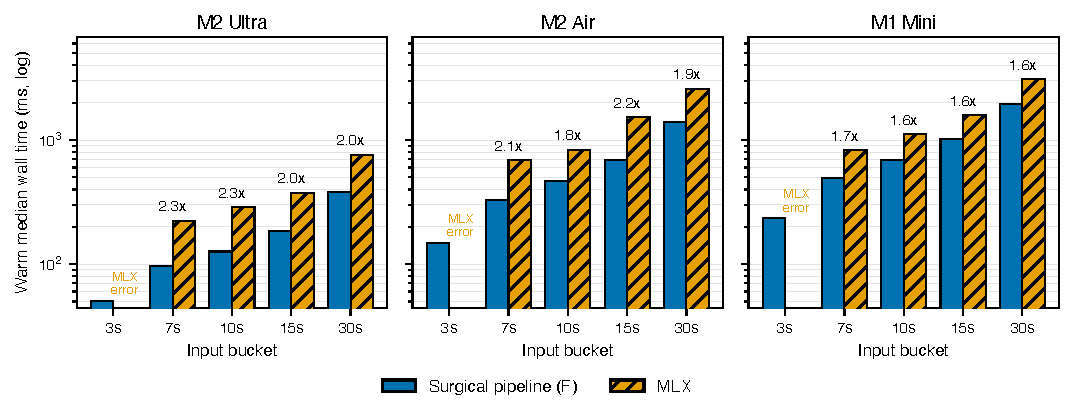
\includegraphics[width=\linewidth]{fig-cs1-latency}}{\pendingfig{fig-cs1-latency}}
\caption{Kokoro-82M end-to-end latency, the Surgical pipeline (Config F) vs.\ MLX, warm medians across three Macs and five input buckets (log axis; \S\ref{sec:cs1-mlx}). The Surgical pipeline is faster on every completed cell, by 1.6--2.3$\times$ (annotated), with the gap widest on the newest silicon. The pinned MLX build fails every 3 s input with a broadcast-shape error, so no 3 s comparison exists.}
\label{fig:cs1-latency}
\end{figure}

\begin{table}[h]
\centering
\small
\caption{Warm median wall time, Configuration F vs MLX; MLX 3 s inputs fail with a broadcast-shape error.}
\label{tab:cs1-mlx}
\begin{tabular}{llll}
\toprule
Input & M2 Ultra (F vs MLX) & M2 Air & M1 Mini \\
\midrule
3s  & 50.6 ms vs \emph{error} & 148.0 ms vs \emph{error} & 233.6 ms vs \emph{error} \\
7s  & 96.1 vs 223.9 ms --- \textbf{2.3$\times$} & 330.7 vs 685.6 ms --- \textbf{2.1$\times$} & 492.7 vs 824.0 ms --- \textbf{1.7$\times$} \\
10s & 126.2 vs 288.8 ms --- \textbf{2.3$\times$} & 466.0 vs 835.8 ms --- \textbf{1.8$\times$} & 685.5 vs 1124.3 ms --- \textbf{1.6$\times$} \\
15s & 185.6 vs 376.3 ms --- \textbf{2.0$\times$} & 693.6 vs 1521.0 ms --- \textbf{2.2$\times$} & 1014.9 vs 1589.5 ms --- \textbf{1.6$\times$} \\
30s & 379.3 vs 762.7 ms --- \textbf{2.0$\times$} & 1404.8 vs 2600.3 ms --- \textbf{1.9$\times$} & 1959.4 vs 3077.9 ms --- \textbf{1.6$\times$} \\
\bottomrule
\end{tabular}
\end{table}

The Surgical pipeline is faster on every bucket on every machine, by \textbf{1.6--2.3$\times$}, with the gap widest on the newest silicon. The pinned MLX version fails all 3-second inputs with a broadcast-shape error, so no 3 s comparison is reportable.

\subsection{vs PyTorch (April 2026 Ledger)}\label{sec:cs1-pytorch}

Warm median wall time, milliseconds, counterbalanced A/D/E/F run (Tables~\ref{tab:cs1-pt-ultra}--\ref{tab:cs1-pt-mini}). The Config F build in this ledger predates the June optimizations; its absolute times are higher than \S\ref{sec:cs1-headline} (e.g. 476 ms vs 379 ms for 30 s on M2 Ultra), so the speedups below are lower bounds for the current pipeline. The April canonical input set had four lengths; the 10 s bucket entered the frozen input set with the June bakeoff, so this ledger has no 10 s row.

\begin{table}[h]
\centering
\caption{April 2026 counterbalanced PyTorch ledger, M2 Ultra (64 GB).}
\label{tab:cs1-pt-ultra}
\begin{tabular}{lrrrrrr}
\toprule
Input & A (Python HAR) & D (MPS) & E (CPU) & F (Surgical) & F vs D & F vs E \\
\midrule
3s  & 333 ms & 225 ms  & 409 ms  & \textbf{57 ms}  & 4.0$\times$ & 7.2$\times$ \\
7s  & 329 ms & 412 ms  & 811 ms  & \textbf{124 ms} & 3.3$\times$ & 6.5$\times$ \\
15s & 486 ms & 673 ms  & 1467 ms & \textbf{239 ms} & 2.8$\times$ & 6.1$\times$ \\
30s & 870 ms & 1602 ms & 2714 ms & \textbf{476 ms} & 3.4$\times$ & 5.7$\times$ \\
\bottomrule
\end{tabular}
\end{table}

\begin{table}[h]
\centering
\caption{April 2026 counterbalanced PyTorch ledger, M2 MacBook Air (24 GB).}
\label{tab:cs1-pt-air}
\begin{tabular}{lrrrrrr}
\toprule
Input & A (Python HAR) & D (MPS) & E (CPU) & F (Surgical) & F vs D & F vs E \\
\midrule
3s  & 461 ms  & 739 ms & 723 ms  & \textbf{185 ms}  & 4.0$\times$ & 3.9$\times$ \\
7s  & 771 ms  & 907 ms & 1839 ms & \textbf{396 ms}  & 2.3$\times$ & 4.6$\times$ \\
15s & 1896 ms & \emph{OOM}  & 3737 ms & \textbf{1326 ms} & ---    & 2.8$\times$ \\
30s & 3918 ms & \emph{OOM}  & 7567 ms & \textbf{3021 ms} & ---    & 2.5$\times$ \\
\bottomrule
\end{tabular}
\end{table}

\begin{table}[h]
\centering
\caption{April 2026 counterbalanced PyTorch ledger, M1 Mac Mini (16 GB).}
\label{tab:cs1-pt-mini}
\begin{tabular}{lrrrrrr}
\toprule
Input & A (Python HAR) & D (MPS) & E (CPU) & F (Surgical) & F vs D & F vs E \\
\midrule
3s  & 238 ms  & 492 ms  & 894 ms  & \textbf{157 ms}  & 3.1$\times$ & 5.7$\times$ \\
7s  & 577 ms  & 1038 ms & 2233 ms & \textbf{511 ms}  & 2.0$\times$ & 4.4$\times$ \\
15s & 837 ms  & 1958 ms & 4458 ms & \textbf{692 ms}  & 2.8$\times$ & 6.4$\times$ \\
30s & 1637 ms & 4167 ms & 8934 ms & \textbf{1229 ms} & 3.4$\times$ & 7.3$\times$ \\
\bottomrule
\end{tabular}
\end{table}

Config F wins every cell where the competitor completes. Three observations:

\begin{enumerate}[leftmargin=*]
\item \textbf{vs MPS: 2.0--4.0$\times$ where MPS finishes at all.} PyTorch MPS exhausts memory on the 15 s and 30 s inputs on the 24 GB Air, even running solo --- the MPS allocation pool plus model state crosses the machine's limit on longer buckets. The ``just use the GPU'' default is not merely slower; on consumer memory configurations it does not complete the workload.

\item \textbf{vs CPU: 2.5--7.3$\times$}, with the largest gains on the M1 Mini's long inputs --- exactly where an interactive application is most likely to be unusable on the CPU path.

\item \textbf{vs the Python+Core ML hybrid (A): 1.1--5.9$\times$.} The narrower margin on some cells reflects that Config A already runs the vocoder through Core ML; Config F's advantage there comes from replacing the Python prefix with Core ML + Swift and from eliminating host-side materialization costs. The June optimizations (not in this ledger) widened this margin further.
\end{enumerate}

The M2 Air Config F rows in this ledger include a since-resolved $\approx$2$\times$ regression in the vocoder stage relative to both earlier and later runs on that machine (compare 3021 ms here with 1405 ms in \S\ref{sec:cs1-headline} for the same 30 s input); we report the ledger as collected.

\subsection{vs Other Core ML Ports}\label{sec:cs1-coreml-ports}

The June bakeoff also benchmarked two independent Core ML Kokoro implementations on the same machines and inputs. Both comparisons require boundary caveats, which we state because they change the interpretation:

\begin{itemize}[leftmargin=*]
\item \textbf{laishere/kokoro-coreml} (pinned \code{484907d}) runs a seven-package Core ML chain. Its public benchmark boundary \emph{excludes} G2P and feed preparation, timing only the Core ML chain --- narrower than our token-IDs-to-PCM boundary. Against it, the Surgical pipeline is 2.3--5.0$\times$ faster on every M2 Ultra bucket and wins the 30 s bucket on all three machines, but laishere's chain-only numbers remain 1.1--1.3$\times$ faster on the M1 Mini's short and medium buckets (and roughly tied, within $\pm$5\%, on the M2 Air below 30 s). We treat this as the most credible remaining performance frontier on low-end hardware, not as a closed question.

\item \textbf{soniqo/speech-swift} (pinned \code{0d09a2e}) emits a fixed $\approx$5.0 s audio artifact for every long-bucket input, so its long-bucket timings are not full-duration synthesis and are not comparable. On the only fully comparable cell (3 s), the Surgical pipeline is 1.4$\times$ faster on M2 Ultra and 5.7--7.4$\times$ faster on the Air and Mini.
\end{itemize}

\subsection{On iPhone}\label{sec:cs1-iphone}

The same \code{.mlpackage} files deploy to iOS unchanged. Release-build warm medians (2 warmups discarded, 5 warm calls, median; iOS 26.5; staged compute policy) are given in Table~\ref{tab:iphone}:

\begin{table}[h]
\centering
\caption{iPhone release-build warm medians, staged compute policy, iOS 26.5.}
\label{tab:iphone}
\begin{tabular}{lrr}
\toprule
Input & iPhone 15 Pro Max (A17 Pro) & iPhone 12 Pro (A14) \\
\midrule
3s  & 426 ms (6.6$\times$ RT)  & 864 ms (3.2$\times$ RT)  \\
7s  & 865 ms (7.8$\times$ RT)  & 1625 ms (4.1$\times$ RT) \\
15s & 1860 ms (7.5$\times$ RT) & 3727 ms (3.7$\times$ RT) \\
30s & 3742 ms (7.3$\times$ RT) & 8551 ms (3.2$\times$ RT) \\
\bottomrule
\end{tabular}
\end{table}

Against the MLX Swift Kokoro port (mlalma/kokoro-ios~\citep{kokoro-ios} 1.0.8 --- the Python mlx-audio above does not run on iOS), a Release-build, thermally controlled arm-vs-arm comparison on the A17 Pro (July 2026; each arm run alone after an identical $\approx$14-minute cooldown; 2 warmups discarded, 5 warm calls, medians) shows the Surgical pipeline winning every bucket, by \textbf{1.25--1.44$\times$}. Two methodological findings from this rerun are worth recording. First, an earlier Debug-build comparison had assumed the Debug tax was symmetric across arms; it is not --- the MLX arm gained 1.4--1.6$\times$ from Release compilation while the Core ML arm's wall time barely moved, so Debug-build ratios are not trustworthy even directionally, and the comparison had to be re-collected. Second, on a fanless phone the run \emph{order} is a thermal treatment: back-to-back arm sweeps penalize whichever arm runs second enough to flip the long buckets (a heat-soaked Core ML arm loses 15 s and 30 s at 0.98$\times$ and 0.84$\times$), which is why the headline protocol thermally matches the arms. The rerun's absolute times sit $\approx$5--9\% above the June table on both arms, consistent with day-to-day variance; the ratios are within-run and unaffected. The kokoro-ios API takes raw text, so its timings include a G2P pass ours excludes; measured in isolation, that pass costs 0.17--1.05 ms per input ($\le$0.03\% of MLX wall time) --- a disclosed asymmetry bounded at $\approx$1 ms, far below every observed margin.

On the 4 GB iPhone 12 Pro (June data, Debug builds on both arms) the result is split: the Surgical pipeline wins 3 s, MLX wins the middle buckets ($\approx$1.2$\times$), and MLX cannot complete the 30 s input at all --- the iOS memory watchdog (jetsam) kills it, reproduced twice, while the Surgical pipeline synthesizes 30 s in 8.6 s on the same phone. Given the Debug-tax asymmetry above, the A14 latency ratios should be treated as indicative only --- if anything, Release builds would widen MLX's middle-bucket advantage there. The memory result is build-independent.

Two iPhone-specific findings: the \code{.all} compute policy hard-fails on both phones (Core ML error $-$9 at the duration stage), so iOS \emph{requires} the explicit staged policy that the Mac pipeline also ships; and bounded memory is a first-class constraint on phones --- fixed-bucket Core ML synthesis ran inside the 4 GB jetsam budget where the GPU framework did not.

\subsection{Stage-Level Breakdown}\label{sec:cs1-stages}

Per-stage warm medians on M2 Ultra (April ledger, Config F) are given in Table~\ref{tab:cs1-stages}:

\begin{table}[h]
\centering
\caption{Per-stage warm medians on M2 Ultra (April ledger, Configuration F).}
\label{tab:cs1-stages}
\begin{tabular}{lrrrrrrr}
\toprule
Input & Duration & F0Ntrain & DecoderPre & Alignment & hn-nsf & Trim & Core ML total \\
\midrule
3s  & 10.0 ms & 4.4 ms  & 2.8 ms  & 0.1 ms & 9.3 ms  & 0.2 ms & 28.5 ms  \\
7s  & 14.3 ms & 18.9 ms & 8.3 ms  & 0.3 ms & 23.1 ms & 0.4 ms & 56.6 ms  \\
15s & 28.8 ms & 38.5 ms & 9.7 ms  & 0.7 ms & 46.9 ms & 0.7 ms & 111.6 ms \\
30s & 52.1 ms & 76.8 ms & 16.6 ms & 1.4 ms & 99.6 ms & 1.6 ms & 224.7 ms \\
\bottomrule
\end{tabular}
\end{table}

``Core ML total'' sums all four model predict calls; the GeneratorFromHar residual is therefore $\approx$11 ms at 3 s and $\approx$79 ms at 30 s. Three observations:

\begin{enumerate}[leftmargin=*]
\item \textbf{The pipeline is well-balanced.} No single stage dominates. The three largest line items at 30 s --- hn-nsf (99.6 ms), generator ($\approx$79 ms), and F0Ntrain (76.8 ms) --- are within 30\% of each other.

\item \textbf{The largest single stage runs on the CPU.} hn-nsf cannot be effectively placed on Core ML (export attempts yielded correlation $\approx$ 0.00 due to SineGen's cumulative phase sensitivity), so the methodology routes it to optimized Swift DSP --- which, after the \S\ref{sec:dsp} optimization pass, costs less than the Core ML stages it sits between.

\item \textbf{The gap between summed stages and end-to-end wall time is host-side work} --- bucket padding, tensor materialization, dispatch --- which is why the methodology treats full-wall-clock as the primary metric (\S\ref{sec:host-cost}). The June optimizations (direct HAR-padding fast path, exact-duration models) attacked exactly this residual.
\end{enumerate}

This table predates two current-pipeline changes --- the frame-source phase fast path in hn-nsf and the DecoderPre/hn-nsf concurrency (\S\ref{sec:cs1-procedure}, \S\ref{sec:cs1-swift}) --- so it overstates the serialized hn-nsf cost relative to the shipped code; the \S\ref{sec:cs1-headline} totals include both.

\subsection{Cross-Machine Scaling}\label{sec:cs1-scaling}

Config F wall time relative to M2 Ultra (June bakeoff) is given in Table~\ref{tab:cs1-scaling}:

\begin{table}[h]
\centering
\caption{Configuration F wall time relative to M2 Ultra (June bakeoff).}
\label{tab:cs1-scaling}
\begin{tabular}{lrrr}
\toprule
Input & M2 Ultra & M2 Air & M1 Mini \\
\midrule
3s  & 1.0$\times$ & 2.9$\times$ & 4.6$\times$ \\
7s  & 1.0$\times$ & 3.4$\times$ & 5.1$\times$ \\
10s & 1.0$\times$ & 3.7$\times$ & 5.4$\times$ \\
15s & 1.0$\times$ & 3.7$\times$ & 5.5$\times$ \\
30s & 1.0$\times$ & 3.7$\times$ & 5.2$\times$ \\
\bottomrule
\end{tabular}
\end{table}

Scaling is smooth and roughly duration-independent above the smallest bucket: the Air sits at $\approx$3.5$\times$ the Ultra's wall time and the Mini at $\approx$5.2$\times$, with no collapse on long inputs and per-bucket RTF nearly flat on each machine (\S\ref{sec:cs1-headline}). The load-bearing finding is that the Surgical pipeline remains comfortably real-time on the lowest-specification machine for inputs up to 30 seconds.

\subsection{Control: A Valid Monolithic Core ML Export Does Not Exist}\label{sec:cs1-monolith}

The natural null hypothesis against decomposition is the monolith: convert the whole model to a single Core ML package, load it under one compute policy, and let the scheduler partition the graph. We tested it directly (coremltools 8.3.0, torch 2.6.0, M2 Ultra; full protocol and verbatim logs in the repository's experiment note, Appendix~\ref{app:artifacts}). It fails at two independent seams --- each one a boundary the decomposed pipeline already cuts:

\begin{itemize}[leftmargin=*]
\item \textbf{The full token-IDs-to-waveform graph does not convert.} The duration-dependent expansion (\code{torch.repeat\_interleave} driven by per-token \emph{predicted} durations) has no static-shape lowering; \code{coremltools} aborts with \code{ValueError: Cannot add const [None]} while converting the op. \code{torch.jit.trace} appears to succeed only by baking one utterance's alignment into constants: the traced graph reproduces its own trace input at correlation 1.000 and hard-crashes on a same-shape input with different predicted durations (\code{The size of tensor a (65400) must match the size of tensor b (67200)}). It is a recording of one utterance's geometry, not a model.

\item \textbf{The strongest partial monolith is numerically invalid.} Fusing every stage downstream of alignment into one package --- aligned features to waveform, including the hn-nsf harmonic source and iSTFT --- converts cleanly and produces wrong audio: correlation 0.27 (FP16) and 0.25 (FP32) against the PyTorch reference. FP32 being equally wrong rules out precision; eager-PyTorch cross-seed correlation of 0.996 rules out RNG mismatch. The divergence is structural, in Core ML's execution of the SineGen cumulative-phase path --- the same failure that forced hn-nsf into native Swift (\S\ref{sec:cs1-swift}, \S\ref{sec:cs1-stages}).
\end{itemize}

There is therefore no single-package latency row to report: for this model, decomposition is not one deployment option among several but the enabling move --- the only route to a correct, compilable on-device Core ML artifact at all. The comparisons in \S\ref{sec:cs1-mlx}--\S\ref{sec:cs1-coreml-ports} (eager GPU frameworks and other \emph{decomposed} Core ML ports) are the strongest baselines that exist.

\section{Case Study 2: Magenta RealTime 2 --- Autoregressive Streaming Under a 40 ms Deadline}\label{sec:cs2}

\subsection{The Workload and the Real-Time Contract}\label{sec:cs2-workload}

MRT2's per-frame loop (\S\ref{sec:mrt2-bg}) must complete in under 40 ms, every frame, indefinitely. The targets were fixed before any conversion work: p50 $<$ 30 ms and p99 $<$ 40 ms per frame, $\ge$ 10 minutes of sustained generation with zero audible dropouts, and sub-200 ms response to control changes. Note what changes relative to Case Study 1: there is no ``bucket'' to finish and no real-time \emph{factor} to maximize. The success metric is a sustained zero-underrun stream, p99 against a wall-clock deadline, and thermal behavior over minutes --- the regime where the ANE's power profile is supposed to beat the GPU.

Applying \S\ref{sec:procedure}'s classification to the per-frame graph (Table~\ref{tab:cs2-motifs}):

\begin{table}[h]
\centering
\caption{Per-frame motif classification of the MRT2 graph.}
\label{tab:cs2-motifs}
\begin{tabularx}{\linewidth}{lXl}
\toprule
Stage & Structure & Motif \\
\midrule
Temporal transformer & 12 layers, d=1024, 8 heads; 41-frame local-attention K/V caches (self + cross) per layer & Sequential-Dynamic \\
Depth transformer & 2 layers, d=768; 12 \emph{serial} RVQ levels per frame, each conditioned on the previous level's sampled token & Sequential-Dynamic \\
Sampling & temperature, top-k, Gumbel noise, per-level valid-range masks, RNG state & Data-Dependent Logic \\
RVQ detokenization & 12 codebook gathers + summation & Data-Dependent Logic \\
SpectroStream decoder & 17 conv2d + 7 conv2d\_transpose, fixed shapes, tokens $\rightarrow$ STFT-rate features & Dense-Static \\
iSTFT / overlap-add & windowed synthesis to PCM, streaming carry & DDL / DSP \\
MusicCoCa prompt encoding & text $\rightarrow$ embedding $\rightarrow$ 12 RVQ style tokens $\rightarrow$ conditioning & off the hot path (control-rate) \\
\bottomrule
\end{tabularx}
\end{table}

One structural decision was made before any export and pays off throughout: \textbf{audio-rate tensors never enter a Core ML graph.} The codec decoder stops at STFT-rate features and host code (Accelerate) performs iSTFT and overlap-add. The Kokoro vocoder's fatal geometry problem (\S\ref{sec:disc-ane}) --- waveform-length axes that exceed ANE admission limits --- is designed out rather than fought.

\textbf{Setup.} The same two iPhones as \S\ref{sec:cs1-iphone}: iPhone 12 Pro (A14, iOS 26.5) and iPhone 15 Pro Max (A17 Pro, iOS 26.5). Conversion went through minimal PyTorch wrappers reconstructed from the released safetensors and validated against the upstream MLX reference, then \code{torch.jit.trace} $\rightarrow$ \code{mlprogram}, FP16 except where noted, minimum deployment target iOS 18. Every export was gated on numerical parity against MLX before any timing was trusted (transformer output correlations $>$ 0.9999; codec decoder SNR $\ge$ 115 dB; token-level sampling parity checked separately). Placement claims below come from \code{MLComputePlan} per-op reports and, for the composed runtime, Instruments traces on the physical phones --- never from the requested compute-unit policy alone.

\subsection{The Pipeline}\label{sec:cs2-pipeline}

Per frame, the shipped pipeline runs: host conditioning assembly $\rightarrow$ Core ML temporal transformer step $\rightarrow$ Core ML depth rollout (samples all 12 RVQ levels in one prediction from host-supplied noise; \S\ref{sec:cs2-bandwidth}) $\rightarrow$ host RVQ codebook summation $\rightarrow$ Core ML codec decoder (overlapping 5- or 25-frame buckets) $\rightarrow$ host iSTFT/overlap-add $\rightarrow$ lock-free SPSC ring $\rightarrow$ \code{AVAudioSourceNode}. The pipeline is shown in Figure~\ref{fig:mrt2-pipeline}. The render callback makes one C call into the ring and never blocks on the model. Generation runs ahead of playback behind a PCM reservoir with high-watermark backpressure: the producer sleeps when the ring is full instead of generating unboundedly.

\begin{figure}[H]
\centering
\IfFileExists{figures/fig-mrt2-pipeline.pdf}{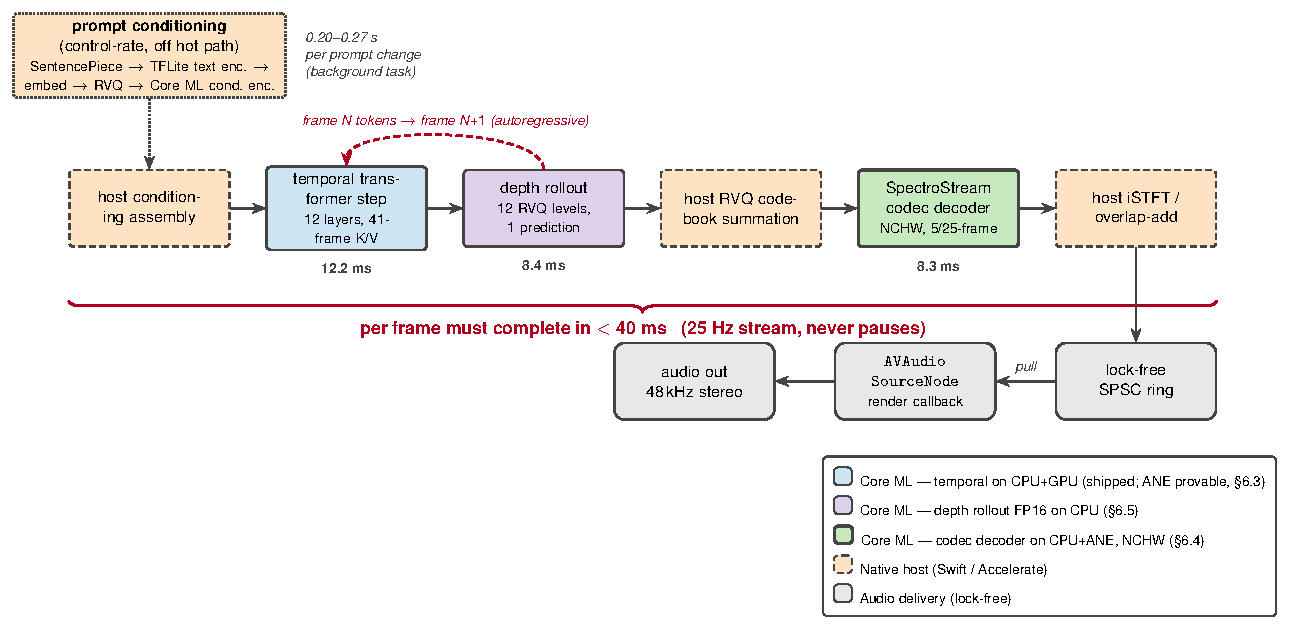
\includegraphics[width=\linewidth]{fig-mrt2-pipeline}}{\pendingfig{fig-mrt2-pipeline}}
\caption{The Magenta RealTime 2 per-frame streaming loop. Every frame must complete within the 40 ms (25 Hz) audio deadline, which never pauses. Audio-rate tensors never enter a Core ML graph --- the codec decoder stops at STFT-rate features and the host synthesizes PCM --- and the three Core ML stages ship on three different engines (temporal on GPU, depth rollout FP16 on CPU, NCHW codec decoder on ANE; per-stage p50 on A17 Pro shown). Generation runs ahead of playback through a lock-free SPSC ring feeding an \code{AVAudioSourceNode}; the render callback never blocks on the model.}
\label{fig:mrt2-pipeline}
\end{figure}

Prompt conditioning is a separate control-rate chain compiled entirely on device --- SentencePiece tokenizer $\rightarrow$ TFLite text encoder $\rightarrow$ embedding mapper $\rightarrow$ RVQ quantizer $\rightarrow$ Core ML conditioning encoder --- running in 0.20--0.27 s steady state per prompt change on both phones, on a background task off the render path. The chain is byte-identical across A14 and A17 Pro at every integer token stage, an unusually strong cross-device determinism property that made it possible to certify with fixture parity rather than statistical testing. A quantization footnote with a generalizable lesson: FP16 on the text encoder preserved all 28/28 test prompts' RVQ tokens byte-exactly (mapped-space drift $7\times10^{-5}$), while int8 dynamic quantization shifted tokens on 8/28 prompts (drift $2\times10^{-3}$) --- \textbf{integer token boundaries downstream of an encoder are the real quantization gate}, not embedding-space error norms.

The per-stage placement story, unlike Case Study 1's, cannot be stated as one clean table --- it is the subject of the next three subsections, and the honest answer differs between ``what was proven possible'' and ``what ships today.''

\subsection{Finding: State Mutation, Not Attention, Is the ANE Cliff}\label{sec:cs2-state}

The \S\ref{sec:motifs} taxonomy assigns the temporal transformer to CPU/GPU. The 25 Hz deadline made that assignment worth attacking, and the attack produced the paper's sharpest finding.

The obvious route is Core ML's mutable state (\code{MLState}) holding the K/V caches. It fails in two ways. A one-frame stateful step \emph{does} compile, with a real ANE island (\code{MLComputePlan}: $\approx$70\% of estimated cost on ANE) --- but every multi-frame unroll fails ANE compilation (\code{MILCompilerForANE ... ANECCompile() FAILED}, error $-$14): the full 2/4/8/16/25-frame matrix on the A17 Pro, and the 25-frame artifact on both phones. And the one-frame graph that compiles is not even a latency win under streaming pressure: 25 sequential \code{MLState} predictions on the A14 measure p99 29.7 ms per call, against 14.7 ms for the same graph CPU-only. A first host-owned-cache export --- which still assembled cache updates in-graph --- also failed ANE compilation. At this point the folklore conclusion (``streaming transformers don't fit the ANE'') was fully available, and wrong.

Instead of concluding, we ran a falsification ladder: strip the graph to one suspect mechanism, prove it on device, add the next suspect back. Each rung is a separate \code{.mlmodelc}, measured on the iPhone 12 Pro with \code{MLComputePlan} placement evidence (FP16, p99 over warmed runs), summarized in Table~\ref{tab:cs2-ladder} and Figure~\ref{fig:ane-ladder}:

\begin{figure}[H]
\centering
\IfFileExists{figures/fig-ane-ladder.pdf}{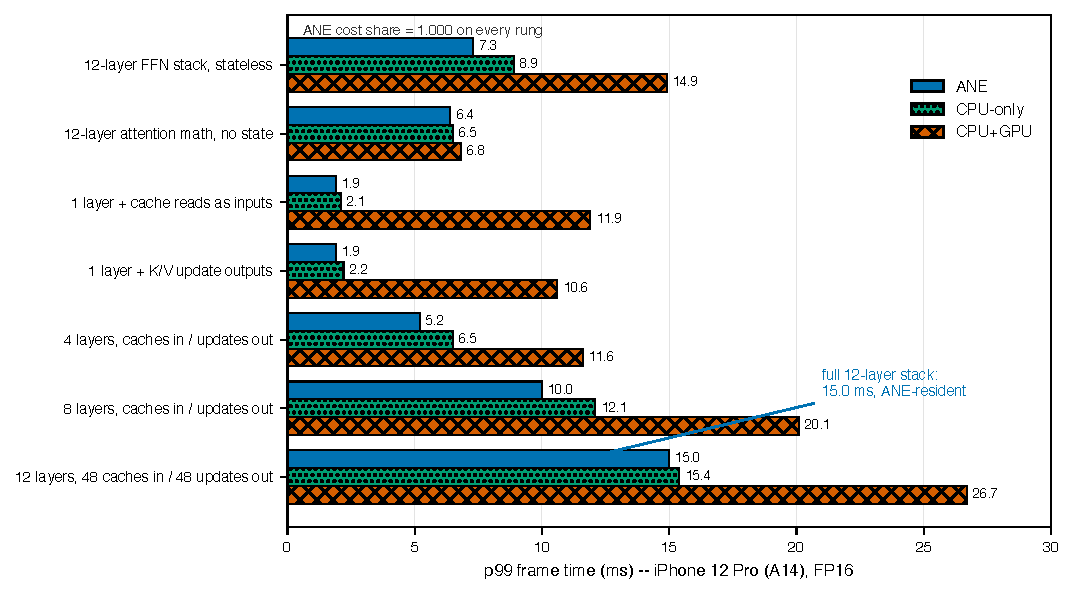
\includegraphics[width=\linewidth]{fig-ane-ladder}}{\pendingfig{fig-ane-ladder}}
\caption{The falsification ladder that located the ANE admission cliff for streaming transformers (p99 per frame, iPhone 12 Pro / A14, FP16; \S\ref{sec:cs2-state}). Every rung is ANE-clean (ANE cost share 1.000) and the ANE placement beats both CPU-only and CPU+GPU --- including the complete 12-layer stack with all 48 K/V caches read in and 48 one-token updates written out, at 15.0 ms. The one thing that must be absent is in-graph cache mutation: attention, softmax, concatenation, and update outputs are all admissible; the state write is the cliff.}
\label{fig:ane-ladder}
\end{figure}

\begin{table}[h]
\centering
\small
\caption{Falsification ladder: p99 per rung across compute-unit policies, iPhone 12 Pro (A14), FP16; every rung ANE cost share 1.000.}
\label{tab:cs2-ladder}
\begin{tabular}{@{}p{5.6cm}rrrr@{}}
\toprule
Graph & ANE cost share & p99 ANE & p99 CPU-only & p99 CPU+GPU \\
\midrule
12-layer FFN stack, stateless & 1.000 & 7.3 ms & 8.9 ms & 14.9 ms \\
12-layer attention math, no state & 1.000 & 6.4 ms & 6.5 ms & 6.8 ms \\
1 layer + cache reads as inputs & 1.000 & 1.9 ms & 2.1 ms & 11.9 ms \\
1 layer + current-token K/V update outputs & 1.000 & 1.9 ms & 2.2 ms & 10.6 ms \\
4 layers, caches in / updates out & 1.000 & 5.2 ms & 6.5 ms & 11.6 ms \\
8 layers, caches in / updates out & 1.000 & 10.0 ms & 12.1 ms & 20.1 ms \\
\textbf{12 layers, 48 caches in / 48 one-token updates out} & \textbf{1.000} & \textbf{15.0 ms} & 15.4 ms & 26.7 ms \\
\bottomrule
\end{tabular}
\end{table}

Every rung is ANE-clean. The complete temporal stack --- all attention, all FFN, all cache reads, all per-token cache-update outputs --- compiles to a single ANE-resident graph (the only CPU ops are zero-cost casts) and beats both CPU-only and GPU placement, provided one thing is absent: \emph{in-graph cache mutation}. Attention matmuls, softmax, concatenation against cache tensors, even forty-eight update outputs are all admissible; the cliff is the state write. Restated for the taxonomy: the recurrence in a streaming transformer is cache \emph{bookkeeping} --- Data-Dependent Logic that belongs to the host --- wrapped around per-step math that is Dense-Static. Cut at that boundary and the motif assignment inverts. Core ML becomes a stateless temporal-math accelerator; Swift/C++ owns cache storage, the shift-and-append, and continuity.

Honesty about where this stands in the shipped app: the cliff has teeth beyond compile time. The stateless-boundary artifact that ran cleanly in the headless runtime host (including a 10-minute zero-underrun streaming proof, \S\ref{sec:cs2-power}) later hit a compiler failure with silent CPU fallback ($\approx$640 ms/frame) inside the full application context, and the numerically \emph{correct} rolling-cache stateful graph that replaced it during a correctness overhaul (\S\ref{sec:cs2-host}) reproduces ANECCompile $-$14 on the A14 in both of its variants --- both of which mutate caches in-graph, consistent with the finding. The shipped temporal placement is therefore \code{.cpuAndGPU} today, with the proven stateless boundary as the documented escape to re-land. Every graph that mutated cache state inside Core ML failed admission; every graph that did not, passed --- but admission is also \emph{instance-fragile}, and a placement that passed in a test harness must be re-proven in the shipping process.

\subsection{Finding: Layout Determines Numerical Survival, Not Just Placement}\label{sec:cs2-layout}

The SpectroStream decoder is textbook Dense-Static: fixed-shape 2D convolutions and transposed convolutions. The naive FP16 export compiled --- and produced non-finite output (finite ratio 0.71). The failure localized to the large parallel transposed-convolution upsampling tail; an FP32 variant was numerically clean but scheduled entirely onto the CPU at roughly 8$\times$ the latency the ANE would eventually deliver. The fix was neither precision nor op rewriting but \emph{internal memory layout}: converting the upsampling block to channels-first (NCHW) internally while preserving the public channel-last I/O contract. The result, on the iPhone 12 Pro (FP16, \code{MLComputePlan} + on-device output-health checks), is given in Table~\ref{tab:cs2-decoder}:

\begin{table}[h]
\centering
\small
\caption{SpectroStream decoder placement and FP16 output health, iPhone 12 Pro.}
\label{tab:cs2-decoder}
\begin{tabular}{llrl}
\toprule
Decoder artifact & Policy & p99 & Output finite? \\
\midrule
5-frame, channels-last FP16 & any & --- & \textbf{no} (0.71 finite ratio) \\
5-frame, NCHW FP16 & \code{.cpuAndNeuralEngine} (ANE 1.000) & \textbf{6.7 ms} & \textbf{yes} (30,720/30,720) \\
5-frame, NCHW FP16 & CPU-only & 27.8 ms & no (29,056/30,720) \\
5-frame, NCHW FP16 & CPU+GPU & 32.2 ms & no (29,056/30,720) \\
25-frame, NCHW FP16 & \code{.cpuAndNeuralEngine} (ANE 1.000) & \textbf{24.8 ms} & \textbf{yes} (184,320/184,320) \\
25-frame, NCHW FP16 & CPU-only & 152.7 ms & no \\
\bottomrule
\end{tabular}
\end{table}

Two lessons. First, the placement win is large ($\approx$4--6$\times$ over CPU) and total: the NCHW artifact schedules every executable op onto the ANE, including the \code{slice\_by\_index}/\code{conv\_transpose} pattern that the channels-last version pushed to CPU. Second, channels-first internal layout is documented vendor guidance for ANE \emph{throughput}~\citep{apple-ane-transformers}; what we have not seen documented is the numerical coupling: \textbf{the ANE was the only compute unit that produced finite output from the same FP16 artifact.} Placement and numerics are not independent axes: each engine runs a different lowering of the same MIL program, with different accumulation and layout paths, and FP16 survival can differ across them. ``Validate numerically, per placement, on device'' is not paranoia; for this stage it was the difference between music and NaNs.

This finding complements Case Study 1's op-rewrite null result (\S\ref{sec:disc-ane}): there, source-level rewrites suggested by ANE folklore changed nothing because the binding constraint was tensor geometry; here, a layout rewrite changed everything because the binding constraint was the FP16 numerical path. The constant is that only a per-stage, on-device ablation tells you which regime you are in.

\subsection{Finding: Weight Bandwidth Is the Invariant That Shapes the Graph}\label{sec:cs2-bandwidth}

The depth transformer samples 12 RVQ levels per frame, serially --- level $k$ conditions on the token sampled at level $k-1$. The natural deployments are 12 small predictions per frame (full pass or stateful step). Both were built, both validated token-for-token, and both cost the same on device: $\approx$40--45 ms/frame on the A14 --- over the entire frame budget --- whether the call computes 12 positions or one.

The explanation is a single number. Every Core ML prediction streams the stage's full weights from DRAM: 97 MB (FP32 depth weights) $\div$ 3.4--3.8 ms per call $\approx$ 26--29 GB/s --- the A14's LPDDR4X bandwidth. Cross-check: the 364 MB FP16 temporal graph measures 13.9 ms isolated, the same $\approx$26 GB/s. \textbf{Per-call cost $\approx$ weight bytes $\div$ DRAM bandwidth, on every compute unit.} Twelve calls per frame means twelve weight streams ($\approx$1.2 GB/frame); no scheduler, compute unit, or state representation can fix that. It also reframes the ANE-vs-GPU question for bandwidth-bound stages: neither engine manufactures bandwidth, so latency parity is expected and the ANE's case rests on power (\S\ref{sec:cs2-power}).

The fix that respects the invariant moves the 12-level autoregressive rollout \emph{inside} one prediction, so weights stream once per frame --- while keeping determinism host-owned, the methodology's standing rule for sampling. The host supplies per-level Gumbel noise \code{[12, 1024]} and inverse temperature as inputs (host RNG and seeds preserved; Gumbel-max~\citep{astar-sampling} over a static top-k set is distributionally identical to top-k softmax sampling); top-k and valid-range masks are constants; the embedder feedback between levels is an in-graph gather reading 12 rows. Measured depth cost per frame: 37 ms FP32 $\rightarrow$ \textbf{12.7 ms FP16 on A14, 8.4 ms on A17 Pro} --- bytes $\div$ bandwidth, as predicted. The FLOAT32 export is token-exact against the reference (0/900 mismatches across autoregressive chains); FP16 flips near-tie tokens without changing the distribution, and was shipped after instrumented and paired-listening gates.

This is the methodology absorbing a new rule rather than breaking: \S\ref{sec:procedure}'s ``sampling stays on CPU'' was always about \emph{determinism and dynamism}, not geography. When bandwidth makes call count the binding constraint, sampling logic can move into the graph as long as the entropy source and the validation gates stay host-owned.

\subsection{Finding: Host Glue Can Silently Destroy Correctness}\label{sec:cs2-host}

Case Study 1's host-side bugs cost milliseconds (\S\ref{sec:host-cost}). This case study's cost music, and they motivate the validation rules now folded into the procedure. Three bugs shipped in early device builds while every model-level validation passed:

\begin{itemize}[leftmargin=*]
\item \textbf{Strided output misread.} Core ML pads output rows for 64-byte alignment: the depth logits tensor \code{[1, 12, 12294]} carries strides \code{[147648, 12304, 1]} --- 10 padding elements per row. The Swift sampler indexed \code{level $\times$ (count / 12)}, so level $k$ read logits shifted by $10\cdot k$ positions. Level 0 was correct (coarse structure always sounded plausible); levels 1--11 sampled from misaligned logit slots --- scrambled fine detail, collapsed stereo. Every Python-side validation passed because \code{coremltools} honors strides; the Swift read path was never validated. Found by an RNG-free argmax A/B that diverged at frame 0, level 1, with matching logit \emph{values} at offset indices.
\item \textbf{Feedback that never existed.} The runtime allocated the temporal feedback input once, zeroed, and never wrote it; and it made one depth prediction per frame where the contract requires 12 autoregressive levels. The transformer graphs were faithful; the loop around them did not implement the model.
\item \textbf{Write-only state.} The one-frame stateful temporal graph baked an attention bias that masked \emph{all 41 history slots}: it wrote K/V state every frame and never read it. Teacher-forced parity and within-prediction unroll parity both pass on a write-only state --- the graph ran for weeks with no self-attention history before a fresh-vs-warmed-state bit-identity test exposed it.
\end{itemize}

The resulting process rules are now part of step 6 of the procedure: every host-side consumer of an \code{MLMultiArray} must be validated against a Python reference at least once, reads must go through \code{strides} rather than \code{count $\div$ dims}, and a stateful graph is not validated until a cross-prediction test proves the state is \emph{read} (same input on fresh vs. warmed state must differ, and an N-prediction stateful drive must match a streaming reference past the window size). After the fixes, the device output joins the reference cluster: left-right correlation 0.99 (matching the MLX reference), prompt-adherence embedding scores within the clean reference band, and blind automated listening gates passing at the shipped temperature with known-bad controls correctly rejected.

\subsection{Placement, Power, and Residency Evidence}\label{sec:cs2-power}

Case Study 1 stated ANE residency as policy intent (a limitation, \S\ref{sec:disc-limitations}). This case study instruments it directly, and the instrumentation is itself a contribution: requested compute units are a \emph{request} (\S\ref{sec:gpu-centric}), and this workload produced multiple concrete demonstrations --- \code{.cpuAndNeuralEngine} artifacts whose compute plan was 100\% CPU, and an \code{.all} policy that mapped a stage entirely to the slower GPU.

\textbf{Residency.} Instruments Core ML traces on both phones, with the all-ANE policy, show per-model ANE hardware intervals for all three model families (on the A17 Pro: temporal 1,729 predictions averaging 7.8 ms of ANE time; depth 0.55 ms; decoder 18.9 ms) and a Metal GPU interval table containing \emph{only} the system compositor --- zero rows attributed to the app process. The check is encoded as a machine-readable gate: a placement-evidence artifact that requires ANE prediction intervals for every model family and rejects any app-attributed GPU interval, so future regressions fail a verifier rather than a vibe.

\textbf{Power.} Paired Power Profiler captures on the A14 --- identical graphs and workload, only the temporal stage's compute policy varied --- show the all-ANE policy at process \code{gpuImpact} 0.000 / \code{cpuImpact} 1.38 / 48.1 B CPU instructions over 60 s, against the temporal-GPU control at 2.23 / 2.63 / 110.3 B. The ANE policy removes process-attributed GPU impact entirely and cuts CPU instructions by 56\%. In the same comparison the producer's \emph{duty cycle} tells the thermal story: the ANE arm finished each second of audio fast enough to sleep 43\% of the run under backpressure; the GPU arm worked 93\% of wall-clock to deliver the same stream. (These captures predate the \S\ref{sec:cs2-host} correctness fixes; both arms ran the identical semantics, so the policy-controlled comparison stands, but the absolute throughput numbers do not transfer to the corrected pipeline.) On the A17 Pro, process-level power impact did \emph{not} separate the policies --- the Instruments residency trace was required to prove placement there, which is why the methodology treats power tables and residency traces as complementary rather than alternative evidence. Figure~\ref{fig:power} plots the paired power metrics.

\begin{figure}[H]
\centering
\IfFileExists{figures/fig-power.pdf}{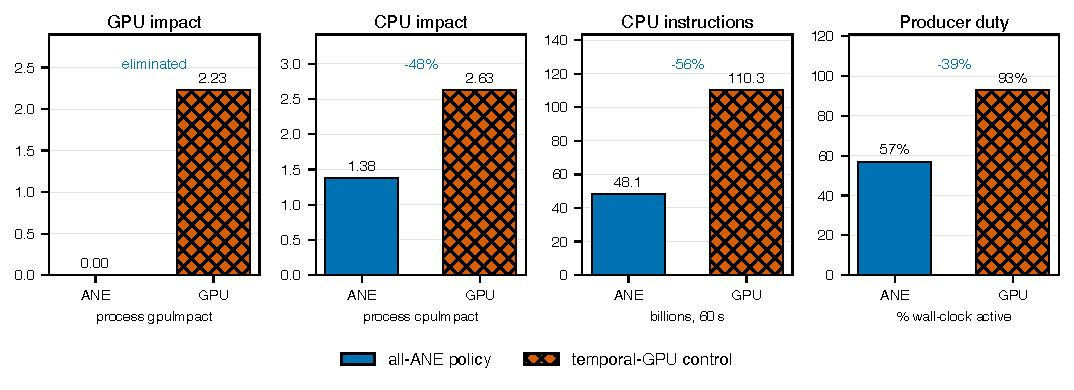
\includegraphics[width=\linewidth]{fig-power}}{\pendingfig{fig-power}}
\caption{Paired power comparison on the A14 (iPhone 12 Pro), all-ANE temporal policy vs.\ a temporal-GPU control running identical graphs over 60 s (\S\ref{sec:cs2-power}). The ANE policy eliminates process-attributed GPU impact entirely (2.23 $\rightarrow$ 0.000) and cuts CPU instructions by 56\% (110.3 B $\rightarrow$ 48.1 B), while the producer's duty cycle drops from 93\% to 57\% --- it finishes each second of audio fast enough to sleep 43\% of the run under backpressure.}
\label{fig:power}
\end{figure}

\textbf{End-to-end status, stated plainly.} With the corrected, numerically verified pipeline (rolling temporal on GPU, in-graph depth rollout FP16 on CPU, NCHW decoder on ANE): the iPhone 15 Pro Max runs faster than real time --- composed $\approx$29 ms/frame p50 (temporal 12.2 + depth 8.4 + decoder 8.3), zero underruns over bounded 45 s runs with backpressure engaged, $\approx$1.37$\times$ real-time headroom. The iPhone 12 Pro does not currently hold the budget ($\approx$50 ms/frame; combined temporal+depth DRAM traffic is $\approx$0.7 GB/frame, $\approx$67\% of the A14's bandwidth --- \S\ref{sec:cs2-bandwidth}'s invariant again). And the 10-minute \emph{foreground} sustain gate currently fails on the A17 Pro: both arms of a controlled soak bank $\approx$20 s of ring lookahead and then thermal-throttle to $\approx$0.95$\times$ real time around minutes 5--7, screen on, with the UI's Metal load included. The earlier 10-minute zero-underrun runs (headless host, all-ANE placement, pre-fix producer) validated the delivery architecture --- SPSC ring, reservoir, backpressure --- but not the corrected pipeline's thermal envelope. The named open work is exactly what the findings predict: re-land the temporal stack on the ANE via the stateless host-cache boundary (\S\ref{sec:cs2-state}), and cut temporal weight bytes (\S\ref{sec:cs2-bandwidth}). We report the gap rather than the trend line.

\section{Discussion}\label{sec:discussion}

\subsection{Why Does the Kokoro Pipeline Win?}\label{sec:disc-why}

The Surgical pipeline's advantage over GPU-only frameworks has six sources:

\begin{enumerate}[leftmargin=*]
\item \textbf{A better scheduling unit.} The original model is not the natural unit of deployment. It contains several computational regimes with different hardware affinities. Once those regimes become separate artifacts, the runtime can schedule them independently instead of forcing the whole graph through one backend.

\item \textbf{Ahead-of-time compiled static graphs.} Each Core ML stage is a fixed-shape fp16 graph, compiled and fused once at load. MLX and PyTorch MPS dispatch eager Metal kernels per op. For a pipeline executed thousands of times with identical shapes, AOT compilation wins even on the \emph{same} silicon --- the generator runs on CPU+GPU through Core ML and still beats the Metal-eager baselines.

\item \textbf{Elimination of Python.} PyTorch MPS incurs interpreter cost between operations; five \code{model.forward()} calls through the GIL cost real milliseconds. The Surgical pipeline is Swift end-to-end.

\item \textbf{Avoidance of MPS fallback overhead.} PyTorch MPS lacks certain operations (notably \code{aten::angle}, used in STFT), forcing per-op CPU round-trips. The Surgical pipeline implements hn-nsf natively in Swift and never pays this cost.

\item \textbf{Cross-unit concurrency.} Because the stages are separate artifacts with explicit dataflow, the CPU-bound hn-nsf source runs on a background thread \emph{during} the DecoderPre Core ML predict (\S\ref{sec:cs1-procedure}). A monolithic graph executes serially on whatever unit the scheduler picked; the decomposition turns one of the largest CPU stages into partly hidden time.

\item \textbf{ANE participation where the ANE admits the graph.} DecoderPre loads with \code{.cpuAndNeuralEngine} and is the one stage whose geometry fits ANE constraints. This is a real but partial contribution; per-stage ablations on the losing machines showed that moving \emph{other} stages to CPU+ANE either failed validation or ran slower.
\end{enumerate}

This is also why the methodology matters for concurrent workloads. A GPU-only Kokoro occupies the GPU for the entire synthesis path. Surgical Inference still uses the GPU for stages that measure best there, but it shortens the total wall time, moves some work to CPU/ANE, exposes idle windows, and avoids routing irregular DSP through the GPU. That is the path to keeping the GPU available for another local workload such as an LLM. We have not yet run a co-scheduling benchmark with TTS and an LLM; the claim here is architectural headroom, not a measured throughput result. Case Study 2 supplies the first direct measurement of the underlying property: under its all-ANE policy, the generating process shows zero attributed Metal GPU intervals and zero process GPU power impact while streaming audio (\S\ref{sec:cs2-power}).

We did not run controlled ablations isolating each factor's contribution --- and \S\ref{sec:cs1-monolith} shows the cleanest such ablation, a monolithic Core ML baseline, cannot exist for this model: conversion fails at the alignment seam, and the strongest partial monolith is numerically invalid. The per-stage compute-unit ablation data (which motivated the staged policy) is the closest available evidence, and it suggests factors 1--5 dominate. We state the missing factor-isolation as a limitation (\S\ref{sec:disc-limitations}), but the \S\ref{sec:cs1-monolith} control also sharpens the paper's central honest finding: \textbf{the win comes from decomposition and native orchestration, not from any single accelerator --- and for this model, decomposition is not merely faster but the precondition for a correct Core ML artifact existing at all.}

\subsection{The ANE Admission Findings}\label{sec:disc-ane}

An earlier draft of this work assumed the Dense-Static stages would run on the ANE under \code{compute\_units=ALL}. The evidence says otherwise, and the correction matters for anyone applying this methodology:

\begin{itemize}[leftmargin=*]
\item \textbf{The vocoder categorically exceeds ANE tensor limits.} GeneratorFromHar's harmonic input has a last-axis extent of 28,801--288,001 elements across the buckets and its waveform output 72,000--720,000 --- far beyond the $\approx$16,384 per-axis limit documented by the community and confirmed by our own compiler errors (\code{Tensor width goes beyond limit supported (16390 $>$ 16384)}).

\item \textbf{Forcing it fails loudly on every machine; \code{.all} fails silently.} Loading the generator with \code{.cpuAndNeuralEngine} fails ANE compilation (\code{MILCompilerForANE ... ANECCompile() FAILED}) on every Mac tested, and the fallback execution runs $\approx$54$\times$ slower than CPU+GPU ($\approx$1517 ms vs $\approx$28 ms on M2 Ultra, 3 s bucket --- an isolated single-model \code{predict()} benchmark used for this placement ablation, distinct from the $\approx$11 ms figure in \S\ref{sec:cs1-stages}, which is the generator's marginal share of full end-to-end wall time obtained by subtracting the other three models' costs from the observed pipeline total, not a second measurement of the same call). Under \code{.all}, macOS silently reroutes the rejected subgraph --- the model ``works'' and the developer learns nothing. iOS is stricter: \code{.all} hard-fails at predict time on both test iPhones.

\item \textbf{The shipped policy is therefore explicit and staged}: DecoderPre on \code{.cpuAndNeuralEngine}; Duration, F0Ntrain, and GeneratorFromHar on \code{.cpuAndGPU}. The same policy runs on Mac and iPhone, which makes the cross-device numbers policy-matched.

\item \textbf{Surface-level graph surgery did not change placement.} We tested rewrites suggested by ANE reverse-engineering literature --- \code{nn.Linear} $\rightarrow$ 1$\times$1 \code{Conv1d}, native instance-norm lowering, broadcast-AdaIN reformulation, fp16 input dtypes, palettization --- against the fused generator. All passed strict numerical validation; none produced a material runtime improvement, and the Linear$\rightarrow$Conv1d change was reverted. The MIL compiler appears to make these lowering decisions itself; the binding constraint is tensor geometry, not op selection.
\end{itemize}

The generalizable lesson: \emph{Dense-Static is the candidate set for the ANE, not a guarantee.} Audio-rate tensors need either re-chunking along the time axis to fit admission limits --- future work --- or the honest fallback this paper ships: Core ML-compiled CPU+GPU execution, which is already faster than the eager GPU frameworks.

Across the two case studies, three \emph{distinct} binding constraints governed ANE admission, and none is documented as such by the vendor:

\begin{enumerate}[leftmargin=*]
\item \textbf{Tensor geometry} (Case Study 1): waveform-rate axes exceed per-axis limits; no op rewrite helps because the constraint is shape, not lowering. Case Study 2 routed around this by construction --- its codec graph stops at STFT-rate features and the host synthesizes PCM.
\item \textbf{In-graph state mutation} (Case Study 2, \S\ref{sec:cs2-state}): every temporal graph that mutated K/V cache state inside Core ML failed \code{ANECCompile}; the identical math as a stateless step function compiled clean and beat CPU and GPU. The escape is a boundary redesign, not an op substitution.
\item \textbf{FP16 lowering paths coupled to layout} (Case Study 2, \S\ref{sec:cs2-layout}): the same FP16 program produced finite output on the ANE and non-finite output on CPU and GPU after a channels-first rewrite --- and was non-finite everywhere before it. Admission here is not binary compile success but numerical survival, per compute unit.
\end{enumerate}

The two case studies also disagree instructively about rewrites: Kokoro's op-level rewrites (Linear $\rightarrow$ 1$\times$1 conv, norm lowerings) changed nothing, while MRT2's layout rewrite changed everything. Both are consistent with one rule: the MIL compiler already makes op-level lowering decisions, so source cosmetics are no-ops, but \emph{structural} properties --- shapes, state boundaries, memory layout --- are the developer's lever, and only a per-stage on-device ablation reveals which structural property is binding.

\subsection{When Surgical Inference Is Worth the Effort}\label{sec:disc-worth}

Surgical Inference required substantial engineering: per-bucket Core ML exports with numerical validation, a Swift package with custom DSP, per-stage compute-unit ablations, and a counterbalanced bakeoff harness. This effort is justified when:

\begin{itemize}[leftmargin=*]
\item \textbf{The workload is compute-bound and parallelizable.} Dense convolutional vocoders, image denoisers, and speech encoders fit. Memory-bandwidth-bound autoregressive transformers do not.
\item \textbf{The pipeline has distinct stages.} A single undifferentiated block offers fewer decomposition opportunities. Models with encoders, decoders, samplers, DSP, token logic, or post-processors are better candidates.
\item \textbf{Target hardware spans a range of devices.} The advantage is decisive on constrained hardware: MPS OOMs on a 24 GB laptop, and MLX is jetsam-killed on a 4 GB phone, where the bucketed Core ML pipeline completes.
\item \textbf{Real-time or interactive constraints matter.} For offline batch synthesis on a workstation, PyTorch MPS may be sufficient. For an app that must synthesize speech while rendering UI or running an assistant model, freeing GPU time matters. Case Study 2 is the limiting case: under a hard streaming deadline, the methodology's per-stage placement and host-owned glue are not an optimization but the only viable shape.
\end{itemize}

The methodology is less useful for:

\begin{itemize}[leftmargin=*]
\item LLM inference (memory-bandwidth-bound; the ANE provides no bandwidth advantage --- and Case Study 2's bandwidth invariant, \S\ref{sec:cs2-bandwidth}, quantifies exactly why)
\item Small one-shot models where Python overhead is already negligible
\item Research contexts where PyTorch flexibility outweighs deployment performance
\end{itemize}

\subsection{Applicability to Other Workloads}\label{sec:disc-applicability}

The empirical claims of this paper now cover two structurally different generative systems: a feed-forward batch TTS pipeline (Kokoro-82M) and a hard-real-time autoregressive streaming music model (MRT2). The second port is evidence that the decomposition procedure (\S\ref{sec:procedure}) is not TTS-specific: the same motif classification, the same per-stage ablation, and the same host-glue discipline produced a working pipeline in a regime with no buckets, no batch boundary, and a stateful transformer on the hot path. Beyond these two:

\begin{itemize}[leftmargin=*]
\item \textbf{Speech and audio.} Other TTS architectures, neural codecs, source-filter vocoders, speech enhancement, and Whisper-style encoder-decoders all mix dense neural blocks with DSP, masking, or sequence logic. The ANE admission analysis (\S\ref{sec:disc-ane}) transfers directly: vocoders that emit audio-rate tensors need time-axis chunking or host-side synthesis from feature-rate tensors (the route Case Study 2 took), and streaming encoders with cache state should be exported as stateless step functions (\S\ref{sec:cs2-state}).
\item \textbf{Image and video generation.} Encoders, denoisers, VAE decoders, schedulers, safety checkers, and post-processing often have different hardware affinities. Dense fixed-shape blocks are natural Core ML candidates; schedulers and dynamic post-processing belong in native code.
\item \textbf{Agentic local assistants.} A local LLM may remain on GPU because it is memory-bandwidth-bound, while speech I/O, wake-word models, embedding models, rerankers, image encoders, and audio decoders can be decomposed away from the GPU. The useful question is not ``can the LLM run on ANE?'' but ``which surrounding stages can leave the GPU alone?'' Case Study 2's power data (\S\ref{sec:cs2-power}) is the existence proof that a nontrivial generative workload can stream continuously with zero process GPU impact.
\end{itemize}

\subsection{Limitations}\label{sec:disc-limitations}

\textbf{Residency and power instrumentation is asymmetric across case studies.} Case Study 1's published runs have no Instruments Core ML timelines or power traces; its staged policy states placement \emph{intent} (the iPhone \code{.all} rejection proves the scheduler honors stage policies), but the fraction of DecoderPre actually executing on ANE silicon is unmeasured. Case Study 2 closes this gap for its own pipeline --- per-model ANE hardware intervals, app-attributed-GPU-absence checks, and paired Power Profiler captures (\S\ref{sec:cs2-power}) --- and that tooling should be back-ported to the Kokoro benchmarks.

\textbf{Case Study 2's power comparison predates its correctness fixes.} The paired ANE-vs-GPU power captures ran identical graphs in both arms, so the policy-controlled deltas (GPU impact removed, CPU instructions $-$56\%) stand, but the absolute duty cycles were measured on a producer later found semantically incorrect (\S\ref{sec:cs2-host}) and do not transfer to the corrected pipeline.

\textbf{Case Study 2's sustained envelope is open.} The corrected pipeline is faster than real time on the A17 Pro over bounded runs but fails the 10-minute foreground soak by thermal throttling to $\approx$0.95$\times$ real time (screen on, UI Metal load included), and the A14 is above the frame budget entirely ($\approx$50 ms/frame). The named fixes --- re-landing the temporal stack on the ANE via the stateless boundary, and cutting temporal weight bytes --- are motivated by the \S\ref{sec:cs2-state}/\S\ref{sec:cs2-bandwidth} findings but not yet demonstrated. ANE admission also proved \emph{instance-fragile}: an artifact that compiled to the ANE in a test harness later fell back to CPU inside the shipping app (\S\ref{sec:cs2-state}), so placement must be re-proven per process, not per artifact.

\textbf{No concurrent workload benchmark.} We have not yet measured synthesis while a local LLM runs on the GPU. The paper's GPU-headroom argument follows from shorter wall time, staged placement, partial CPU/ANE execution, and Case Study 2's zero-GPU-impact traces, but it needs a direct co-scheduling benchmark before becoming a throughput claim.

\textbf{MPS fallback overhead in Config D.} Config D uses \code{PYTORCH\_ENABLE\_MPS\_FALLBACK=1}, the realistic developer default, so its timings include CPU fallback costs for unsupported ops. The MLX comparison (\S\ref{sec:cs1-mlx}) partially addresses this --- MLX is a fallback-free Metal path and the Surgical pipeline still wins by 1.6--2.3$\times$ --- but a fallback-free MPS variant was not benchmarked.

\textbf{Two-vintage results.} The PyTorch ledger (April) and the MLX/external bakeoff (June) used different builds of Config F; the April speedups are conservative for the current pipeline but are not contemporaneous with \S\ref{sec:cs1-headline}. The April M2 Air rows additionally contain a since-resolved vocoder regression, disclosed in \S\ref{sec:cs1-pytorch}.

\textbf{Remaining frontier on low-end hardware.} laishere's chain-only Core ML numbers remain faster than our full-pipeline numbers on M1 Mini short/medium buckets (\S\ref{sec:cs1-coreml-ports}). Graph-surface replication experiments (\S\ref{sec:disc-ane}) did not close this gap; the difference likely lies in runtime placement, weight decompression, or boundary structure, and is unresolved.

\textbf{Audio quality evaluation is automated, not human --- and it caught real defects that per-stage parity certified as correct.} To move beyond informal listening checks, we ran a structured perceptual evaluation of Case Study 1's shipped pipeline: the PyTorch eager reference (float32, CPU) versus the Swift + Core ML pipeline under its shipped staged compute policy, on the four frozen benchmark inputs (2.8--27.4 s), judged by a multimodal audio model (Gemini) in blind paired lineups with a known-bad control and repeat-vote agreement, alongside the objective waveform gate. The initial run passed the short and medium buckets cleanly --- the judge rated the Core ML output ``perceptually indistinguishable'' from the reference while unambiguously rejecting a speech-shaped static control that the objective waveform gate cannot catch --- and failed both long buckets: 3/3 votes on ``unnatural silent gaps'' at 15 s, and 2/2 votes on ``background static and hiss'' at 30 s, backed by signal analysis (phrase pauses measured 40--110 ms long; 1--9 kHz energy at 0.35--0.48$\times$ of the gain-matched reference). Stage-boundary tensor bisection traced both to implementation defects invisible to per-stage matched-input correlation: a native post-process that silenced punctuation-adjacent whitespace spans carrying real speech ($-$11 to $-$22 dBFS word onsets and phrase-final decays), and an export-time inverse-STFT substitution that scaled every interior frequency bin of the one-sided spectrum at half amplitude --- a defect present in \emph{every} bucket and every compute policy, which the judge only flagged where exposure was longest. A third, compounding defect surfaced during root-causing rather than from the perceptual gate directly: the Swift harmonic-source noise generator's xorshift64 RNG had an absorbing zero state, so the fixed seed used for every evaluated clip produced a degenerate DC-and-Nyquist-only ``noise'' signal instead of broadband Gaussian noise, muting the harmonic source across the board and compounding the iSTFT amplitude bug specifically at the seed used for every reported clip. After fixing all three (suppression narrowed to punctuation tokens; corrected one-sided iSTFT weights re-exported, matching the reference generator to $5\times10^{-7}$ max abs; the RNG reseeded via SplitMix64 scrambling so no seed reaches the absorbing state), all four inputs pass the blind evaluation (15 s 2/2, 30 s 2/2) and the control is still rejected. This is an automated model-judged evaluation, not a human MOS study: it establishes reproducible end-to-end perceptual parity on the frozen inputs and demonstrated the discriminative power to catch three shipped defects, but it does not calibrate absolute quality scores. Commands, verdicts, signal analyses, and the root-cause chain are recorded in the repository (Appendix~\ref{app:artifacts}). Case Study 2 reports token-level parity, embedding-space adherence and stereo-correlation metrics against the MLX reference, and blind automated listening gates with known-bad controls --- also short of a formal MOS study, and its adherence scores sit below the upstream runtime-CFG reference because the on-device pipeline bakes guidance at export time.

\textbf{Single-vendor evaluation.} All measurements are on Apple Silicon. The motif taxonomy and the decomposition procedure do not assume Core ML, but the constraint catalog (\S\ref{sec:disc-ane}) is Apple-specific; other NPU toolchains (Qualcomm QNN, LiteRT delegates) impose different admission rules and would need their own per-stage ablations before the quantitative claims transfer.

\textbf{Hardware coverage.} Macs: M1, M2, M2 Ultra; iPhones: A14, A17 Pro (both case studies use the same two phones). M3/M4 Macs and A18/A19-class phones were not tested.

\section{Related Work}\label{sec:related}

\textbf{Core ML deployment of large models.} Apple has published a Core ML conversion of Stable Diffusion~\citep{apple-stable-diffusion} and vendor guidance for ANE-friendly transformer deployment~\citep{apple-ane-transformers}; the latter documents channels-first layout conventions as a throughput optimization, which our \S\ref{sec:cs2-layout} finding extends to a numerical-survival condition. In the speech domain, whisper.cpp~\citep{whispercpp} added a Core ML encoder path alongside its Metal decoder, and WhisperKit~\citep{whisperkit} is the closest prior system to our methodology: it decomposes Whisper into per-stage Core ML models with compute-unit selection and ships them in production on Apple devices. These are model-specific engineering efforts; our work adds an explicit cross-model methodology (motif classification, per-stage placement ablation, host-glue validation rules), documents the admission constraints that make the ablation necessary, and validates the method on two structurally different generative workloads with negative results included.

\textbf{Live music generation on device.} Magenta RealTime and its successor MRT2~\citep{magenta-rt,magenta-rt-repo} are, to our knowledge, the first open-weights live-music models with a real-time streaming contract; the upstream deployment path is MLX on M-series Macs, with desktop standalone and plugin surfaces. We are not aware of prior work running this model class in real time on a phone, nor of prior documentation of the state-mutation ANE admission cliff (\S\ref{sec:cs2-state}) or the layout-dependent FP16 survival result (\S\ref{sec:cs2-layout}) that doing so surfaced; Apple's stateful-model documentation~\citep{mlstate} describes the \code{MLState} API but does not specify ANE admission behavior for graphs that mutate state in-graph. The SpectroStream codec follows the residual-vector-quantization lineage of SoundStream~\citep{soundstream}.

\textbf{Core ML Kokoro ports.} laishere/kokoro-coreml~\citep{laishere} runs a seven-package ANE-resident Kokoro vocoder chain and is the strongest prior art for this specific model; we benchmark against it directly (\S\ref{sec:cs1-coreml-ports}) and adopt its chain-only boundary caveat when comparing. soniqo/speech-swift~\citep{speech-swift} ships a Core ML Kokoro for iOS with a fixed-length output artifact. mlalma/kokoro-ios~\citep{kokoro-ios} is the MLX Swift port we compare against on-device (\S\ref{sec:cs1-iphone}).

\textbf{On-device TTS.} Piper~\citep{piper} targets edge deployment with CPU-only inference. MeloTTS~\citep{melotts} provides real-time multilingual synthesis on CPU. These systems prioritize compatibility over performance; hardware-aware decomposition on Apple Silicon buys a further order of magnitude.

\textbf{MLX for Apple Silicon.} MLX~\citep{mlx} provides a NumPy-like GPU interface for Apple Silicon. MLX is complementary to our work: Sequential-Dynamic stages of a larger pipeline could use MLX while Dense-Static stages use Core ML. Our measurements (\S\ref{sec:cs1-mlx}, \S\ref{sec:cs1-iphone}) characterize where the Core ML path wins for convolutional TTS today, including the memory-bounded regime where MLX fails outright.

\textbf{Reverse engineering the ANE.} The Orion project~\citep{orion} and community field guides~\citep{ane-field-guide} document reverse-engineered ANE constraints (per-dispatch overheads, tensor geometry limits, preferred lowerings). Our experiments corroborate the geometry limits as binding for audio-rate tensors, and find that source-level op rewrites suggested by this literature (e.g. Linear $\rightarrow$ 1$\times$1 conv) do not change Core ML runtime performance --- the MIL compiler already makes those decisions (\S\ref{sec:disc-ane}). Case Study 2 adds two constraints this literature does not document: in-graph state mutation as a compile-time admission cliff for streaming transformers, and FP16 numerical survival that differs across compute units as a function of internal layout (\S\ref{sec:disc-ane}).

\textbf{Heterogeneous accelerator scheduling.} The problem of mapping computation to heterogeneous accelerators has been studied extensively in CPU/GPU systems (StarPU~\citep{starpu}, Legion~\citep{legion}) and data-center contexts (TPU/GPU/CPU). In mobile deployment, delegate-based runtimes (ExecuTorch~\citep{executorch}, LiteRT/NNAPI) partition a single graph across NPU backends at runtime. Our contribution applies heterogeneous-scheduling principles to consumer SoCs for multi-stage generative inference, with two differences: the partition is an explicit, measured design artifact rather than a runtime decision, and one accelerator's admission behavior is opaque and must be probed empirically per stage.

\section{Conclusion}\label{sec:conclusion}

We presented Surgical Inference, a methodology for decomposing generative models into smaller neural submodels and native stages that can be scheduled across a heterogeneous SoC, and evaluated it on two structurally opposite workloads. By classifying stages into three computational motifs --- Sequential-Dynamic, Data-Dependent Logic, and Dense-Static --- matching each to candidate hardware, and resolving final placement with per-stage measurement, we produced a Kokoro-82M pipeline that is 1.6--2.3$\times$ faster than MLX, 2.0--4.0$\times$ faster than PyTorch MPS where MPS completes at all, and 2.5--7.3$\times$ faster than PyTorch CPU, across three Macs spanning the consumer-to-workstation range --- and that ships unchanged to iPhone, where it beats the MLX Swift port on current hardware and completes workloads that exhaust the GPU framework's memory budget.

The same procedure carried Magenta RealTime 2 --- a 230M-parameter autoregressive streaming music model whose upstream real-time path requires an M-series Mac GPU --- onto iPhone hardware, and in doing so sharpened the methodology itself. The Sequential-Dynamic motif turned out to be divisible: a streaming transformer is Dense-Static math wrapped in cache bookkeeping, and cutting at that boundary --- caches as inputs, one-token updates as outputs, host-owned mutation --- moved the complete 12-layer stack through an ANE compiler that rejects every stateful variant. Layout proved to govern numerical survival, not just speed: after a channels-first rewrite, the ANE was the only compute unit producing finite FP16 codec output. And weight bandwidth emerged as the invariant that shapes graph boundaries on phones: per-call cost is weight bytes over DRAM bandwidth on every engine, which collapsed a twelve-prediction sampling loop into one in-graph rollout fed by host-supplied noise. Instruments traces and paired power profiles did what policy flags cannot --- proved all-ANE residency with zero app-attributed GPU time and a 56\% cut in CPU instructions against a GPU control. The corrected pipeline runs faster than real time on an iPhone 15 Pro Max; the 10-minute thermal envelope and the A14 budget remain open, and we report them as open.

The methodology argues that the prevailing ``use the GPU'' convention in local inference is suboptimal for compute-bound generative pipelines with distinct stages. It also corrects the inverse oversimplification: the Neural Engine is not a magic substrate that dense graphs simply run on. A single-package Core ML export of the first case study cannot validly exist (\S\ref{sec:cs1-monolith}); the ANE rejected that case study's largest dense stage on geometry, rejected the second's transformer whenever state mutation entered the graph, and was simultaneously the only engine that ran the second's codec correctly. The win survives in both cases because decomposition --- static per-stage graphs, native orchestration, deliberate placement, and validated host glue --- is the active ingredient, with each accelerator contributing where its admission constraints allow.

Across both case studies, the right question for on-device AI is not ``which single accelerator should run this model?'' The better question is: ``what is the smallest set of static neural packages and native kernels that lets the whole chip execute the workload?'' That framing is what makes faster, more efficient, less GPU-monopolizing local inference possible --- for batch synthesis on hardware people already own, and for generative audio that streams in real time from the phone in their pocket.

\bibliographystyle{plainnat}
\bibliography{refs}

\appendix
\section{Artifact and Reproduction Map}\label{app:artifacts}

\subsection{Case Study 1 (Kokoro-82M)}

The implementation artifacts for the first case study are in the open-source \code{kokoro-coreml} repository:

\begingroup\let\code\pth
\begin{itemize}[leftmargin=*]
\item Swift runtime pipeline: \code{swift/Sources/KokoroPipeline/}
\item Main pipeline loader and staged compute-unit policy: \code{swift/Sources/KokoroPipeline/KokoroPipeline.swift}
\item End-to-end synthesis executor and DecoderPre/hn-nsf overlap: \code{swift/Sources/KokoroPipeline/KokoroSynthesisExecutor.swift}
\item Direct token-to-frame expansion: \code{swift/Sources/KokoroPipeline/MLMultiArrayHelpers.swift}
\item Harmonic source DSP implementation: \code{swift/Sources/KokoroPipeline/HarmonicSource.swift}
\item Waveform trim and punctuation suppression: \code{swift/Sources/KokoroPipeline/WaveformPostProcess.swift}
\item Mac bakeoff harness: \code{scripts/bakeoff\_harness.py}
\item External bakeoff adapters: \code{scripts/external\_bakeoff/}
\item iPhone benchmark app: \code{ios-bench/}
\item Monolithic-export control experiment (\S\ref{sec:cs1-monolith}), protocol and verbatim logs: \code{README/Notes/monolithic-coreml-control-experiment.md}
\item Structured perceptual evaluation (\S\ref{sec:disc-limitations}), protocol, verdicts, and signal analyses: \code{README/Notes/cs1-audio-quality-evaluation-2026-07-14.md}
\item Release-build iPhone comparison (\S\ref{sec:cs1-iphone}), thermal protocol and raw results: \code{README/Notes/iphone-release-build-mlx-comparison.md}
\item Per-cell dispersion verification run (\S\ref{sec:cs1-setup}), protocol and raw data: \code{README/Notes/config-f-dispersion-run-2026-07-14.md}
\end{itemize}
\endgroup

The pre-converted Core ML packages are published with the repository release artifacts and on the project Hugging Face model page.

\subsection{Case Study 2 (Magenta RealTime 2 / Crossfade)}

The conversion and validation layer is public in the \href{https://github.com/mattmireles/magenta-realtime-2-iphone}{\code{magenta-realtime-2-iphone}} repository and covers both artifact generations:

\begingroup\let\code\pth
\begin{itemize}[leftmargin=*]
\item Corrected exporters reproducing the \S\ref{sec:cs2-state}--\S\ref{sec:cs2-bandwidth} findings: \code{exporters/convert\_temporal\_body\_carry.py} (stateless host-owned-cache temporal boundary, \S\ref{sec:cs2-state}), \code{exporters/convert\_depth\_body\_rollout.py} (in-graph FP16 depth rollout, \S\ref{sec:cs2-bandwidth}), and \code{exporters/convert\_spectrostream\_decoder.py --fp16-rescale} (the finite-FP16 channels-first decoder path, \S\ref{sec:cs2-layout})
\item Superseded exporters retained and labeled as negative-result artifacts: running the stateful temporal exporter reproduces the \code{ANECCompile} $-$14 rejection, and the decoder without the FP16-safe path reproduces the non-finite output
\item Numerical-parity validators and validation receipts: \code{validation/} (including the depth rollout's 0/900 token-exactness receipt)
\item Reference fixtures, graph-teardown and KV-cache documentation, and the artifact inventory with tensor contracts: \code{fixtures/}, \code{docs/}, \code{MODELS.md}
\end{itemize}
\endgroup

Pre-built \code{.mlpackage} binaries on the \href{https://huggingface.co/mattmireles/magenta-realtime-2-iphone}{Hugging Face mirror} are the superseded generation at the time of writing; the corrected artifacts are reproducible from the exporters above, and \code{MODELS.md} states per artifact what is uploaded versus reproducible-from-exporter. The streaming runtime and instrumentation live in the \code{crossfade} repository, a fork of \code{magenta/magenta-realtime} that is private at the time of writing (artifacts available from the author). Within it:

\begingroup\let\code\pth
\begin{itemize}[leftmargin=*]
\item Conversion wrappers and exporters: \code{magenta\_rt/coreml/}, \code{scripts/convert\_mrt2\_*.py}, \code{scripts/convert\_spectrostream\_decoder\_*.py}
\item Numerical-parity validators (vs the MLX reference): \code{scripts/validate\_mrt2\_*.py}, \code{scripts/verify\_spectrostream\_streaming\_decode.py}
\item On-device probe used for the falsification ladder and placement matrices: \code{examples/ios/CoreMLMRT2Probe/}
\item Production runtime (stateless temporal boundary, depth rollout, SPSC ring, reservoir/backpressure): \code{Sources/CrossfadeRuntime/}, \code{Sources/CrossfadeRuntimeCore/}
\item Residency-proof runner emitting the machine-checkable \code{placement-evidence.json}: \code{scripts/run\_coreml\_trace\_device.py} with \code{scripts/summarize\_coreml\_xctrace\_exports.py}
\item Paired ANE-vs-GPU power capture with the comparability gate: \code{scripts/run\_power\_profiler\_pair\_device.py} with \code{scripts/summarize\_power\_xctrace\_exports.py}
\item Sustained-run log analyzer (duty cycle, backpressure share, underruns, thermal): \code{scripts/analyze\_crossfade\_runtime\_host\_log.py}
\item Investigation ledgers with per-run device log paths: \code{README/Notes/mrt2-coreml-proof-v1.md}, \code{README/Notes/mrt2-small-graph-teardown-v1.md}
\end{itemize}
\endgroup

\section{Benchmark Boundaries}\label{app:boundaries}

The benchmark boundary used throughout Case Study 1 is:

\begin{verbatim}
phoneme token IDs + voice embedding
    -> full synthesis pipeline
    -> 24 kHz PCM waveform resident in memory
\end{verbatim}

Model download, process startup, first-use Core ML compilation/cache effects, playback, and text-to-phoneme conversion are excluded unless a comparison implementation's public API forces a wider boundary. Such boundary differences are disclosed in \S\ref{sec:cs1-coreml-ports} and \S\ref{sec:cs1-iphone}.

Case Study 2 uses two boundaries appropriate to streaming. Stage and per-frame timings are measured at the Core ML prediction call (warmed, p50/p99 over sustained runs, with \code{MLComputePlan} or Instruments placement evidence attached to the same run). End-to-end claims are measured at the audio contract: frames pushed into and pulled from the render ring by the live \code{AVAudioSourceNode}, with underrun events, dropped frames, ring fill watermarks, and \code{ProcessInfo.thermalState} logged per generation iteration. Sustained results report the full counter set rather than a single latency figure, because a streaming pipeline can have excellent median latency and still fail its product contract at minute seven.

\end{document}
